\documentclass[11pt]{article}
\usepackage[a4paper,margin=24mm,headheight=14pt]{geometry}
\usepackage[T1]{fontenc}
\usepackage[utf8]{inputenc}
\usepackage{lmodern,microtype}
\usepackage{amsmath,amssymb,amsthm,mathtools}
\usepackage{booktabs,longtable,array,tabularx}
\usepackage{enumitem,xcolor,graphicx,tikz}
\usetikzlibrary{arrows.meta,positioning,calc}
\usepackage{fancyhdr}
\usepackage{hyperref}
\definecolor{navy}{HTML}{18334D}
\definecolor{teal}{HTML}{007C83}
\definecolor{pale}{HTML}{F1F6F8}
\hypersetup{colorlinks=true,linkcolor=navy,citecolor=teal,urlcolor=teal,
 pdftitle={Exact binary boundary tensors and compressed transport for unknot recognition},
 pdfauthor={Research prepared for Vladimir Reshetnikov}}
\pagestyle{fancy}
\fancyhf{}
\fancyhead[L]{\small\textcolor{navy}{Unknot recognition: exact compression}}
\fancyhead[R]{\small 8 October 2026}
\fancyfoot[C]{\thepage}
\setlength{\parskip}{4pt}
\setlength{\parindent}{0pt}
\setlength{\emergencystretch}{2em}
\setlist{nosep,leftmargin=*}
\newtheorem{theorem}{Theorem}[section]
\newtheorem{lemma}[theorem]{Lemma}
\newtheorem{proposition}[theorem]{Proposition}
\newtheorem{corollary}[theorem]{Corollary}
\theoremstyle{definition}
\newtheorem{definition}[theorem]{Definition}
\newtheorem{example}[theorem]{Example}
\theoremstyle{remark}
\newtheorem{remark}[theorem]{Remark}
\newcommand{\Z}{\mathbb Z}
\newcommand{\F}{\mathbb F}
\newcommand{\N}{\mathbb N}
\newcommand{\poly}{\operatorname{poly}}
\newcommand{\LCS}{\operatorname{LCS}}
\newcommand{\LCP}{\operatorname{LCP}}
\newcommand{\lcm}{\operatorname{lcm}}
\newcommand{\code}[1]{\texttt{\detokenize{#1}}}
\newcommand{\status}[1]{\textcolor{teal}{\textbf{#1}}}
\newcolumntype{Y}{>{\raggedright\arraybackslash}X}
\allowdisplaybreaks
\title{\textcolor{navy}{Exact binary boundary tensors and\\compressed transport for unknot recognition}\\[6pt]
\large A faster asymptotic bound for full Jones computation,\\
exact compressed word matching, and boundary-lift constraints}
\author{Research prepared for Vladimir Reshetnikov\\
\small ProveIt / Topology / UnknotRecognition}
\date{8 October 2026}
\begin{document}
\maketitle
\begin{abstract}
This continuation develops three exact compression kernels for the maintained
\code{fastunknot} implementation. The main contribution is an explicit
two-state tensor model of the Kauffman bracket, constructed directly from a
spherical planar-diagram rotation system. An integral cochain supplies the
turning of every smoothing circle without constructing a geometric drawing.
Every frontier with $w$ edges has at most $2^w$ binary states, even when the
processed region has several boundary components. An exact integer
specialization recovers the complete Jones polynomial. Combined with the
repository's certified separator order, this improves its implemented
full-polynomial guarantee from
$\poly(n)2^{O(\sqrt n\log(n+1))}$ to
$\poly(n)2^{O(\sqrt n)}$ bit time. Comparable general bounds already occur in
the literature; the contribution is a concrete implementation and its full
correctness and bit-cost analysis.

The other kernels address operations on compressed descriptions. A long
common prefix reduces exact longest-common-substring search to a bounded set
of diagonals and short-period tests on a grammar. A boundary-lift transport
solver represents all compatible maps of a connected dihedral surface cover
by at most two modular progressions, with an additional canonicalization
theorem in the cyclic case. Each result is accompanied by independent checks,
resource semantics, measurements, and explicit limitations. The complete
unknot recognizer still has no proved general quasi-polynomial bound. The
article identifies the precise inference that would be required to obtain
one and proposes research directions that address that inference.
\end{abstract}

\clearpage
\tableofcontents
\clearpage
\section{Scope, baseline, and mathematical status}
\label{sec:overview}

\subsection{The snapshot being extended}

The source baseline is the public ProveIt repository~\cite{proveit-baseline} at commit
\begin{center}\small
\code{8a95834940cf77cdab1b39571ffc102ca8b6bede}.
\end{center}
All paths below are relative to \code{Topology/UnknotRecognition}, unless a
different root is specified. The most recent baseline commit affecting this
subdirectory is
\begin{center}\small
\code{30d58bd311d96af1e49b6c98584b8da526b7adcc}.
\end{center}
The audit included the maintained implementation in \code{fast/}, the
199-page synthesis and its source sections, and the relevant literature.
The delivered patch is against this fixed snapshot; it does not assume that
the moving \code{main} branch remains unchanged.

This distinction matters because the baseline already incorporates many
earlier improvements. These include structural Seifert and braid
certificates, rational-tangle methods, component and homological compression,
exact Potts evaluations, certified separator orders, full Jones recovery,
and compressed group-presentation search. In particular, alphabet and
directed-pair bounds for compressed substrings are already present.
Reimplementing one of those results would not constitute a continuation.

The present work concentrates on three remaining representation costs:

\begin{enumerate}
\item Full Jones evaluation uses equality partitions of frontier colors.
When the number of colors grows with the input, the available bound is a
Bell number. A fixed two-state model removes this source of the logarithmic
factor in the exponent.
\item Two very long compressed words can share both their alphabet and
their directed pairs. If they already agree almost to their ends, the
remaining search can instead be bounded by their short unmatched tails.
\item A compressed surface cover must preserve the identities of boundary
components used in subsequent gluings. Pointed-cover classification alone
does not solve simultaneous constraints on whole boundary lifts.
\end{enumerate}

The first two kernels are connected to callable recognizer paths in the
patch. The boundary kernel extends a geometric data operation; a complete
Lackenby hierarchy implementation does not yet exist in this codebase.

\subsection{What the main theorem says}

Let $n$ be the number of crossings of a validated classical knot diagram.
For an order of its crossings, let $w$ be the largest number of diagram
edges incident to both processed and unprocessed crossings. Then the new
backend computes the full Jones polynomial with at most $2^w$ frontier keys
and in
\begin{equation}\label{eq:main-width}
 \poly(n)2^{O(w)}
\end{equation}
deterministic bit time. The polynomial factor includes exact arithmetic,
normalization, and coefficient recovery. The default ordering wrapper has
$w=O(\sqrt n)$ and polynomial preparation cost, so
\begin{equation}\label{eq:main-sqrt}
 T_{\mathrm{Jones}}(n)=\poly(n)2^{O(\sqrt n)}.
\end{equation}
The unrestricted statement requires disabled local caps and no external
deadline. With limits enabled, an exhausted query yields no polynomial
identity assertion.

The key point is the absence of a common-disk hypothesis. The baseline
correctly rejects the inference that an arbitrary planar scan has
Catalan-many matchings. We do not reintroduce that inference. The new state
space records two orientations per cut edge and uses a linear evaluation
of the bracket. It never claims to preserve every boundary matching as a
distinct object. Section~\ref{sec:tensors} proves the relevant evaluation
identity directly.

\subsection{Attribution and novelty}

The Kauffman bracket and its relation to the Jones polynomial are classical
\cite{kauffman1987}. Singly exponential dependence on diagram width, and
consequent $2^{O(\sqrt n)}$ algorithms for fixed quantum invariants, are
established in work including Maria's theorem \cite{maria2021}. That paper
also addresses the arithmetic cost. Equation~\eqref{eq:main-sqrt} is
therefore an improvement to the maintained implementation and its proved
bound, not a new general complexity theorem for the Jones polynomial.

The development here supplies a small, direct construction from PD data:
an independently checkable integral turning cochain, a binary frontier
contraction, a proof that one cyclotomic phase suffices for each key, and
exact coefficient recovery from integer arithmetic. The word and covering
results are likewise stated as specific kernels and proved in the
generality actually implemented. No claim of historical priority for every
elementary lemma is needed to assess their correctness or usefulness.

\subsection{The quasi-polynomial target remains distinct}

We use \emph{quasi-polynomial} for bounds of the form
$\exp((\log(n+2))^{O(1)})$. The stronger target repeatedly used in this
project is $n^{O(\log n)}=\exp(O(\log^2 n))$.
The new general Jones bound in \eqref{eq:main-sqrt} is subexponential but is
larger than every bound with a fixed power of $\log n$ in the exponent.

Moreover, a full Jones polynomial equal to one is not a recognized unknot
certificate. The baseline explicitly preserves an independent exact
fallback. The patch preserves that behavior. Khovanov homology supplies a
complete detection theorem \cite{kronheimer-mrowka}; this does not bound the
size of the intermediate chain complexes used to compute it.

Lackenby's July 2026 preprint gives a new hierarchy algorithm and
polynomially encoded certification machinery \cite{lackenby2026}. Its
Section~9 separates iteration counts from running time and gives an
iteration bound $L(g+1)^L$ in terms of maximum hierarchy length and pattern
complexity. The refined length control in Section~10 is linear in initial
handle complexity. These results do not provide the complete accelerated
quasi-polynomial implementation sought here. In particular, compressing one
local operation does not bound the number or sizes of future operations.

\subsection{Reading the evidence}

Proofs establish correctness and asymptotic claims. Exhaustive finite
checks test conventions and implementation against independently organized
oracles. Timings measure completed executions on the stated machine; a
resource limit is reported as a limit rather than as a completion time.
Section~\ref{sec:experiments} reports both favorable cases and regressions.
The package contains the patch, complete runnable source, test and audit
drivers, raw measurements, and build instructions.

\section{Integral turning data from a rotation system}
\label{sec:turning}

\subsection{Darts, faces, and smoothing conventions}

Suppose first that $n>0$. A validated PD diagram is a connected four-valent
plane multigraph with $n$ vertices and $2n$ edges. Loops and repeated edges
are allowed. At crossing $v$, its four darts are numbered $(v,0)$ through
$(v,3)$ in counterclockwise order. Write $\sigma(v,j)=(v,j+1\bmod4)$ and
let $\alpha$ exchange the two darts of each edge. The cycles of
\begin{equation}\label{eq:face-permutation}
 \phi=\sigma\alpha
\end{equation}
are the oriented face walks. There are $n+2$ of them, and their total length
is $4n$. A face walk may repeat vertices and edges.

The two smoothings pair slots as follows:
\[
 S_0=\{\{0,1\},\{2,3\}\},\qquad
 S_1=\{\{0,3\},\{1,2\}\}.
\]
Their bracket weights are $A$ and $A^{-1}$, respectively. We use the
unnormalized bracket $\mathcal B_D(A)$, in which every closed circle has
weight $\delta=-A^2-A^{-2}$. Thus
\begin{equation}\label{eq:bracket-state-sum}
 \mathcal B_D(A)=\sum_{s\in\{0,1\}^n}
      A^{n-2|s|}\delta^{c(s)},
 \qquad
 V_D(A^{-4})=(-A^3)^{-\operatorname{wr}(D)}
                   \frac{\mathcal B_D(A)}{\delta}.
\end{equation}
Here $c(s)$ counts the smoothing circles. These conventions agree with the
independent Laurent-polynomial oracle supplied by the baseline.

At a smoothing arc traversed from incoming slot $j$ to outgoing slot $k$,
define its quarter-turn by
\begin{equation}\label{eq:corner-turn}
 \tau(j,k)=
 \begin{cases}
 -1,&k=j+1\pmod4,\\
 +1,&k=j-1\pmod4.
 \end{cases}
\end{equation}
The incoming tangent points into the crossing, which explains the minus
sign in the first case. In particular, each corner of a face walk in
\eqref{eq:face-permutation} has quarter-turn $-1$.

\begin{figure}[ht]
\centering
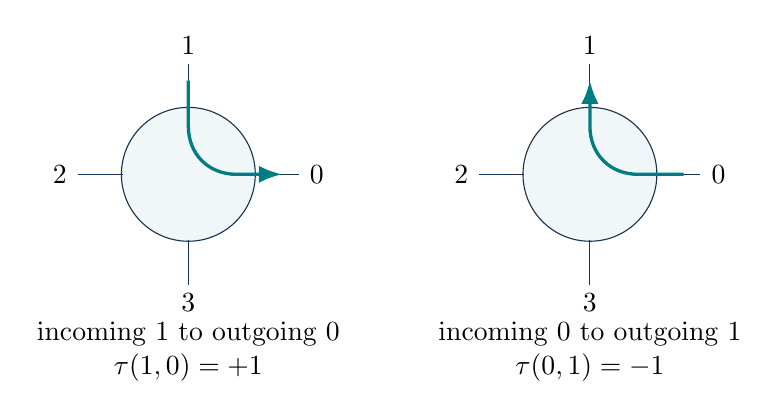
\begin{tikzpicture}[scale=0.85,>=Latex]
 \draw[fill=pale,draw=navy] (0,0) circle (1.0);
 \foreach \a/\s in {0/0,90/1,180/2,270/3}{
  \draw[navy] (\a:0.98)--(\a:1.65);
  \node at (\a:1.92) {$\s$};
 }
 \draw[very thick,teal,->] (0,1.4)--(0,0.72)
  .. controls (0,0.3) and (0.3,0) .. (0.72,0)--(1.4,0);
 \node[align=center] at (0,-2.65) {incoming $1$ to outgoing $0$\\$\tau(1,0)=+1$};
 \begin{scope}[xshift=6.0cm]
 \draw[fill=pale,draw=navy] (0,0) circle (1.0);
 \foreach \a/\s in {0/0,90/1,180/2,270/3}{
  \draw[navy] (\a:0.98)--(\a:1.65);
  \node at (\a:1.92) {$\s$};
 }
 \draw[very thick,teal,->] (1.4,0)--(0.72,0)
  .. controls (0.3,0) and (0,0.3) .. (0,0.72)--(0,1.4);
 \node[align=center] at (0,-2.65) {incoming $0$ to outgoing $1$\\$\tau(0,1)=-1$};
 \end{scope}
\end{tikzpicture}
\caption{The local convention. Slot numbers increase counterclockwise,
but the entering tangent reverses the slot's outward direction.}
\label{fig:turn-convention}
\end{figure}

\subsection{A small system of face equations}

Choose one face $f_\infty$ as the outer face. A directed edge-turn cochain
is a family of integers $b_d$, one for every dart, satisfying
$b_{\alpha(d)}=-b_d$. We require
\begin{equation}\label{eq:turn-equations}
 \sum_{d\in f} b_d=
 \begin{cases}
 |f|-4,&f\ne f_\infty,\\
 |f|+4,&f=f_\infty.
 \end{cases}
\end{equation}
These equations contain the total edge turning along each face; the
$|f|$ local corners contribute $-|f|$ separately.

\begin{theorem}[Constructive integral turning cochain]
\label{thm:turn-construction}
For every connected spherical four-valent rotation system with $n>0$, the
equations \eqref{eq:turn-equations} have an integer solution supported on
the edges dual to a dual spanning tree. Such a solution can be constructed
and verified in polynomial bit time and encoded in $O(n\log(n+2))$ bits.
For the construction used here,
\begin{equation}\label{eq:cochain-bounds}
 \max_d |b_d|\le4n+4,
 \qquad
 L_b:=\sum_{e}|b_e|\le4(n+1)^2.
\end{equation}
The sum over edges chooses either orientation once.
\end{theorem}

\begin{proof}
Put $h_f=|f|-4+8\mathbf1_{f=f_\infty}$. Euler's formula gives
\[
 \sum_f h_f=4n-4(n+2)+8=0.
\]
Choose a spanning tree of the connected dual graph, rooted at $f_\infty$.
For a nonroot face $f$, let $d_f$ be the dart on its parent edge belonging
to $f$. Assign $b_{d_f}$ the total demand of the subtree rooted at $f$ and
assign its negative to the other dart. Assign zero on all remaining edges.
At $f$, its parent-edge contribution is its subtree demand; the
child-edge contributions subtract the children's subtree demands.
Their sum is $h_f$. The root equation follows from total demand zero.
This also handles a primal bridge: its dual loop belongs to no spanning
tree and contributes zero twice with opposite signs.

The total positive demand equals half the absolute demand sum, and
\[
 \sum_f |h_f|\le\sum_f(|f|+4)=8n+8.
\]
Every subtree sum therefore has absolute value at most $4n+4$.
There are $n+1$ dual-tree edges, proving \eqref{eq:cochain-bounds}.
The construction uses face walks, a tree traversal, and integer subtree
sums. Its verifier reconstructs the face walks, checks antisymmetry, and
checks every equation in \eqref{eq:turn-equations}; it does not repeat the
tree construction. All numbers used by the constructed certificate have
$O(\log(n+2))$ bits.
\end{proof}

\subsection{Why every smoothing circle has the right turning}

\begin{lemma}[Zero face integrals determine all closed integrals]
\label{lem:closed-cochain}
Let $c$ be an antisymmetric edge cochain on a connected graph cellularly
embedded in the sphere. If its integral around every face walk is zero,
then its integral around every closed graph walk is zero. The statement
holds over $\Z$ and over $\Z/4\Z$.
\end{lemma}

\begin{proof}
Choose a primal spanning tree. For each nontree edge, its fundamental
cycle bounds a union of faces, with signs determined by orientation.
The integral around that cycle is consequently zero. Define a vertex
potential by integrating $c$ along the tree from a root. The vanishing
fundamental-cycle integrals show that the difference of potentials across
every edge is $c$ on that edge. Potential differences telescope on every
closed walk. This argument uses no division and works over either ring.
Repeated edges on a face boundary cancel with their orientations.
\end{proof}

\begin{theorem}[Turning of all smoothing circles]
\label{thm:turning}
Let $b$ satisfy \eqref{eq:turn-equations}. For any smoothing state, orient
one of its circles $C$ arbitrarily. Sum $b_d$ along its directed traversals
of diagram edges and sum \eqref{eq:corner-turn} along its smoothing arcs.
The resulting integer is $+4$ or $-4$. Reversing $C$ negates the integer.
\end{theorem}

\begin{proof}
Take any smooth planar realization of the rotation system with the chosen
outer face. In small disjoint neighborhoods of its crossings, arrange
the four outward tangents in the cardinal directions indexed by the
slots. This is possible because their cyclic orders agree. Smooth the
remaining edges while keeping those endpoint tangents fixed.
Let $b^{\mathrm{geom}}_d$ be the total tangent turning along such an edge,
measured in quarter-turns. Endpoint tangent directions make this an integer.
It is antisymmetric under reversal.

A slightly regularized face boundary turns once clockwise for an inner
face and once counterclockwise for the outer face. Its local crossing
corners each contribute $-1$. Hence $b^{\mathrm{geom}}$ satisfies exactly
\eqref{eq:turn-equations}, including faces whose combinatorial walks
repeat vertices. By Lemma~\ref{lem:closed-cochain}, the difference
$b-b^{\mathrm{geom}}$ has zero integral on every closed graph walk.

The oriented smoothing circle is a simple smooth plane curve. Its total
tangent turning is $+4$ or $-4$ quarter-turns. Replacing the edge part of
that sum by $b$ leaves the total unchanged: after collapsing the small
crossing neighborhoods, the circle determines a closed graph walk.
It may visit one crossing twice, but the lemma explicitly permits this.
The local smoothing turns are precisely \eqref{eq:corner-turn}.
Reversal negates both the edge and corner contributions.
\end{proof}

This proof uses a geometric drawing only as an existence argument. The
algorithm constructs and verifies integers from the rotation system.
No coordinate drawing, floating-point angle, or numerical winding test
appears in the computation.

\begin{corollary}[Gauge independence]
\label{cor:gauge}
For a fixed outer face, any two solutions of the face equations give the
same total turn on every smoothing circle. Different outer-face choices
also yield the same unoriented loop evaluation $\rho^4+\rho^{-4}$.
\end{corollary}

\begin{proof}
The first assertion is Lemma~\ref{lem:closed-cochain}. For the second,
Theorem~\ref{thm:turning} still gives the two opposite values $\pm4$;
summing over both orientations removes their order.
\end{proof}

\begin{remark}[The sphere hypothesis]
On a higher-genus surface, vanishing face integrals need not imply
vanishing integrals on essential cycles. The construction here therefore
requires validated classical diagrams. It is not a Jones algorithm for
arbitrary virtual diagrams with no additional homological data.
\end{remark}

\section{Binary boundary tensors for the bracket}
\label{sec:tensors}

\subsection{Orient each circle instead of recording its connectivity}

Work initially in a commutative extension of
$\Z[A,A^{-1}]$ containing an invertible element $\rho$ with
\begin{equation}\label{eq:rho-fourth}
 \rho^4=-A^2.
\end{equation}
Then $\rho^4+\rho^{-4}=\delta$. By Theorem~\ref{thm:turning}, the sum of the
weights of the two orientations of any smoothing circle is exactly
$\delta$. Thus every factor $\delta^{c(s)}$ in the bracket state sum can
be evaluated by independently orienting the circles.

Choose a canonical dart $d_e$ on each diagram edge; the implementation
chooses the smaller dart index. A binary edge state gives that edge an
arrow, either in the direction of $d_e$ or against it. Write
$\epsilon_d=+1$ when the arrow points out of the vertex at dart $d$, and
$\epsilon_d=-1$ otherwise. Thus $\epsilon_{\alpha(d)}=-\epsilon_d$.
A smoothing is compatible with these arrows if each of its pairs has one
incoming and one outgoing dart.

For a compatible smoothing $s$ at crossing $v$, let $r_v(s,\epsilon)$ be
the sum of its two local turns. It belongs to $\{-2,0,2\}$. Define the
local crossing tensor and the edge weight by
\begin{align}
 T_v(\epsilon)&=\sum_{\substack{s\in\{0,1\}\\s\text{ compatible}}}
          A^{1-2s}\rho^{r_v(s,\epsilon)},\label{eq:crossing-tensor}\\
 E_e(\epsilon)&=\rho^{\epsilon_{d_e}b_{d_e}}.\label{eq:edge-tensor}
\end{align}
The crossing tensor vanishes unless two darts point in and two point out.
Only six of the sixteen arrow configurations can occur. The two alternating
configurations each support both smoothings; the others support one.

\begin{theorem}[Exact two-state contraction]
\label{thm:binary-tensor}
For a validated nonempty classical knot diagram,
\begin{equation}\label{eq:network}
 \mathcal B_D(A)=
 \sum_{\text{one binary arrow per edge}}
     \prod_v T_v(\epsilon)\prod_e E_e(\epsilon).
\end{equation}
For any crossing order, a direct frontier contraction of this expression
has at most $2^{w_i}$ keys after a prefix whose cut has $w_i$ diagram edges.
No connectivity or disk condition on the prefix is required.
\end{theorem}

\begin{proof}
Expand every sum in \eqref{eq:crossing-tensor}. A nonzero term consists of
a smoothing state and an arrow on each edge such that the arrows extend
coherently through every smoothing arc. This is exactly an independent
choice of orientation for each smoothing circle. Its weight is the
smoothing monomial $A^{n-2|s|}$ times $\rho$ raised to the sum of all local
and edge turns. Summing the orientations of one circle gives
$\rho^4+\rho^{-4}=\delta$. Doing this independently for all circles recovers
\eqref{eq:bracket-state-sum}.

To contract a prefix, sum all arrow variables whose two incident crossings
are processed and retain those with exactly one processed endpoint. The
result is a tensor indexed by the latter binary variables. There are
$2^{w_i}$ assignments. A loop at one crossing has both endpoints processed
together and is summed locally. This is ordinary distributivity in a
finite product of local tensors and does not use a boundary matching.
\end{proof}

\subsection{A continuation statement with its exact scope}

Let $P$ be a set of processed crossings, let $Q$ be its complement, and
fix the same full-diagram turning data. Assign each edge factor to its
canonical endpoint. The contraction of $P$ produces a vector $u_P$ and
that of $Q$ produces the complementary vector $u_Q$ on the same cut
assignments. Their contraction is $\mathcal B_D$.

This gives an exact linear summary for the bracket under the remaining
contraction. It does not imply that the summary preserves the relative
Khovanov complex, nor that it distinguishes every topological tangle.
The distinction explains how the binary state bound can coexist with
large matching sets and with the baseline's lower bounds on explicit
categorified checkpoints. Decategorification can identify data that a
chain-complex computation must retain.

\subsection{One cyclotomic phase per frontier key}

For exact arithmetic we later set $A=B^2$ and $\rho=\zeta B$, where
$\zeta^4=-1$. At first sight every coefficient is a four-coordinate
integer in $\Z[\zeta]$. A stronger statement removes most of that storage.

\begin{lemma}[A vertex potential modulo four]
\label{lem:phase-potential}
For an oriented edge from slot $j$ at vertex $v$ to slot $k$ at vertex $u$,
there is a function $\nu$ on vertices with values in $\Z/4\Z$ such that
\begin{equation}\label{eq:phase-potential}
 b_d+j-k-2=\nu(u)-\nu(v)\pmod4.
\end{equation}
\end{lemma}

\begin{proof}
The expression on the left is antisymmetric modulo four. Around a face,
the next departing slot equals the preceding arriving slot plus one,
modulo four. Consequently $\sum(j-k)=|f|\pmod4$. The face sum of the
left side of \eqref{eq:phase-potential} is therefore
$\sum b_d-|f|=\pm4=0\pmod4$. Apply
Lemma~\ref{lem:closed-cochain} over $\Z/4\Z$ and take its vertex potential.
\end{proof}

\begin{theorem}[Phase determined by the boundary]
\label{thm:one-phase}
Fix a set $P$ of processed crossings and a binary assignment on its cut.
All nonzero monomials contributing to that tensor entry have the same
power of $\zeta$ modulo four. The entry therefore has the form
$c\zeta^r$, with $c\in\Z$ and $0\le r<4$, after the integer
specialization and the nonnegative shifts described below.
\end{theorem}

\begin{proof}
At a crossing, the local turning exponent satisfies
\[
 r_v=\sum_{d=(v,j)}\epsilon_d j\pmod4.
\]
Indeed, an arc from incoming $j$ to outgoing $k$ turns by
$k-j-2\pmod4$; summing two arcs subtracts four.
Every allowed crossing has two incoming and two outgoing darts, so
$\sum_{d\text{ at }v}\epsilon_d=0$. We may consequently add
$\nu(v)\sum\epsilon_d$ without changing the phase.

An internal edge of the prefix contributes, from its two endpoints and
its edge factor,
\[
 \epsilon_d\bigl(b_d+j-k+\nu(v)-\nu(u)\bigr)
       =2\epsilon_d=2\pmod4
\]
by Lemma~\ref{lem:phase-potential}. This contribution is independent of
its arrow. A cut edge contributes only terms determined by its fixed
arrow, its processed endpoint, and the fixed convention assigning its
edge factor. Thus the total phase is fixed by the boundary assignment and
by $P$. The extra powers of $B$ used for denominator clearing have no
$\zeta$ phase. Powers differing by four have opposite signs because
$\zeta^4=-1$, and those signs are absorbed into the integer $c$.
\end{proof}

The implementation stores this phase together with one signed integer.
When terms reach the same key, it checks that their phases agree before
adding their integers. The check is an implementation invariant backed by
the theorem, rather than an assumption that discards other coordinates.
Zero entries are removed. A closed result has phase zero, since every
smoothing circle contributes a multiple of four.

\subsection{The executable contraction}

The contraction uses a deterministic crossing order. At each step it
performs the following operations.
\begin{enumerate}
\item Identify the current cut edges incident to the crossing, cut edges
that survive untouched, newly opened edges, and self-loops.
\item Compile the local arrow table from
\eqref{eq:crossing-tensor}--\eqref{eq:edge-tensor}, summing self-loop
orientations immediately. At most eight smoothing--orientation
contributions occur before equal monomials are aggregated.
\item For each stored boundary key, read its incident arrow bits and
apply the compatible local transitions. Copy the untouched bits and
append the new bits to form the next key.
\item Multiply by the compiled local monomials, merge equal keys using
Theorem~\ref{thm:one-phase}, and remove zero entries.
\end{enumerate}
The local tensors have bounded arity. An arbitrary number of holes in the
processed region changes neither the arity nor the binary dimension of a
cut edge. The implementation's cap counts actual tensor updates, not the
number of smoothing states of the full diagram.

\begin{remark}[Why this does not improve Khovanov automatically]
The evaluation in \eqref{eq:network} is an identity for a Laurent
polynomial. Its signed sums can cancel information that would survive in
homology. Applying the same data reduction to a differential without
proving a homotopy or homology comparison would be invalid. A useful next
problem is to identify precisely which additional data, if any, can be
retained at controlled cost; Section~\ref{sec:research} discusses this.
\end{remark}

\section{Faithful integer evaluation and bit complexity}
\label{sec:encoding}

\subsection{Uniform polynomial bounds}

Write $V_D(t)=\sum_j c_jt^j$ for the Jones polynomial of the input knot.
The following deliberately loose bounds suffice:
\begin{equation}\label{eq:coefficient-bounds}
 \sum_j|c_j|\le4^n,
 \qquad c_j=0\quad\text{if }|j|>2n.
\end{equation}
For completeness, the normalized state sum has $2^n$ terms. Splitting each
of the $n$ crossings increases the number of connected components by at
most one, so $c(s)\le n+1$. The coefficient norm of
$\delta^{c(s)-1}$ is $2^{c(s)-1}\le2^n$. The triangle inequality gives
the first bound. Before collecting terms, the smoothing monomial,
circle powers, and writhe correction have total absolute $A$-degree at
most $n+2n+3n=6n$. The normalized exponents are divisible by four for a
knot, giving the sharper $3n/2$ bound and hence the stated $2n$ bound.

Choose
\begin{equation}\label{eq:integer-base}
 \beta=\left\lceil\frac{2n+2}{8}\right\rceil,
 \qquad B=2^\beta,
 \qquad A=B^2,
 \qquad X=B^8.
\end{equation}
Then $X\ge4\cdot4^n$. These choices depend only on the crossing count.
The backend performs no probabilistic polynomial identity test.

\begin{lemma}[Injectivity of bounded integer evaluation]
\label{lem:balanced-injective}
An integer polynomial whose coefficients have absolute value strictly
less than $X/2$ is uniquely determined by its value at $X$, among
polynomials with coefficients in the balanced digit interval
$[-X/2,X/2)$. The same is true for a Laurent polynomial with a known
finite degree range, after multiplication by a fixed monomial.
\end{lemma}

\begin{proof}
The constant coefficient is the unique representative of the residue
modulo $X$ in the balanced interval. Subtract that coefficient and divide
by $X$, then repeat. The resulting digits determine all coefficients.
The procedure works for negative integers as well. Multiplication by a
known monomial reduces the Laurent case to the ordinary polynomial case.
\end{proof}

The coefficient bounds \eqref{eq:coefficient-bounds} lie strictly inside
the balanced interval. In particular, equality with the integer evaluation
of the polynomial one proves \emph{polynomial} identity, not merely
agreement at an arbitrary evaluation point.

\subsection{Clearing negative powers before contraction}

Set $t=\zeta B$ with $\zeta^4=-1$. A local contribution has exponent
$2(1-2s)+r_v$ in $B$, between $-4$ and $4$. Multiply every crossing
tensor by $B^4$. For each edge $e$, multiply its factor by
$B^{|b_e|}$. The two choices of arrow then have nonnegative $B$-exponents
$|b_e|\pm b_e$. Consequently the complete contraction is
\begin{equation}\label{eq:scaled-bracket}
 S_0=B^{K_0}\mathcal B_D(B^2),
 \qquad K_0=4n+L_b.
\end{equation}
Every local coefficient is a bounded sum of signed monomials
$\zeta^r B^e$ with $e\ge0$. Multiplication by such a monomial is a binary
shift of an integer and a phase/sign update. General multiplication of
two large integer coefficients is unnecessary in the sequential scan.

For normalization the implementation sets
\begin{equation}\label{eq:normalization-shift}
 K=\max(K_0,6n+4),\qquad S=B^{K-K_0}S_0.
\end{equation}
The expected scaled bracket of an unknot of the input writhe $a$ is the
integer
\begin{equation}\label{eq:unknot-scalar}
 U=(-1)^{a+1}(B^8+1)B^{K+6a-4}.
\end{equation}
Its exponent is nonnegative because $a\ge-n$ and $K\ge6n+4$.
It is nonzero. Thus $S=U$ can be tested without division and is equivalent
to $V_D=1$, using the faithful evaluation above.

The empty PD is treated separately. In this project it represents one
crossing-free unknot, whose bracket is $\delta$, rather than an empty
link with bracket one. The implementation returns its full polynomial
one even when the local state and transition caps are zero.

\subsection{Recovering every coefficient}

Let $a=\operatorname{wr}(D)$. By the normalization in
\eqref{eq:bracket-state-sum},
\begin{equation}\label{eq:integer-recovery}
 P:=X^{2n}V_D(X^{-1})
   =\frac{(-1)^{a+1}S\,B^{16n+4-K-6a}}{X+1}.
\end{equation}
If the exponent of $B$ in the numerator is negative, move that power to
the denominator. The quotient is an integer: the left side is an
ordinary integer polynomial evaluated at the integer $X$.
The implementation uses exact division and checks its remainder.

Write $P=\sum_{i=0}^{4n}d_iX^i$ in balanced digits. Equation
\eqref{eq:integer-recovery} and Lemma~\ref{lem:balanced-injective} give
\[
 c_j=d_{2n-j}.
\]
The decoder checks the degree and coefficient bounds, and agreement
between the decoded identity and the direct comparison $S=U$. An identity
query does not run the decoder. A full-polynomial query with $S=U$ returns
$\{0\mapsto1\}$ immediately after validating its normalization.
These checks protect the interface against inconsistent data; the tensor
identity is what establishes the mathematical value of $S$.

\subsection{All intermediate integers have polynomially many bits}

The largest possible total $B$-exponent in an expanded shifted tensor
monomial is at most
\[
 E=8n+2L_b.
\]
There are at most $2^n$ smoothing choices and $2^{2n}$ arrow assignments.
Using the triangle inequality, every intermediate integer coordinate
has at most
\begin{equation}\label{eq:bit-bound}
 \beta(8n+2L_b)+3n+O(1)=O(n^3)
\end{equation}
bits, by Theorem~\ref{thm:turn-construction}. Partial contractions obey
the same bound because all shifted exponents are nonnegative. Final
scaling, the normalization integer, and the division in
\eqref{eq:integer-recovery} also use $O(n^3)$-bit integers.
There are only $O(n)$ output coefficients, each of $O(n)$ bits.

The loose cubic bound is intentional. The observed $L_b$ can be much
smaller than its worst-case quadratic bound, and the implementation
reports it. Improving the cochain's $\ell^1$ norm can reduce large-integer
work without changing any topological argument.

\begin{theorem}[Uncapped full Jones complexity]
\label{thm:full-jones}
For any fixed crossing order of width $w$, the new backend computes the
complete Jones polynomial using at most $2^w$ frontier keys and
$\poly(n)2^{O(w)}$ deterministic bit time. Using the existing certified
separator ordering by default gives
\[
 \poly(n)2^{O(\sqrt n)}
\]
bit time for every classical knot diagram. If a supplied family of
orders satisfies $w=O(\log^2(n+2))$, its full Jones queries run in
$n^{O(\log n)}$ bit time.
\end{theorem}

\begin{proof}
Theorem~\ref{thm:binary-tensor} bounds the number of keys. Each crossing
has bounded arity, hence a bounded number of local transitions per
incoming key. Key extraction and all integer operations cost a polynomial
in $n$, using \eqref{eq:bit-bound}. The integer reconstruction also has
polynomial bit cost, even with schoolbook division.

A collision-free table or a balanced search tree gives
$\poly(n)2^w$ operation accounting. The actual Python implementation uses
a sparse integer-key dictionary. Even the conservative worst case in
which a lookup compares every represented key squares the state factor,
which remains $2^{O(w)}$. Thus the displayed deterministic bound does
not rely on an unproved constant-time hash-table assumption. Input edge
labels are normalized; the cost of reading arbitrary integer labels is
polynomial in their supplied bit length.

The baseline separator constructor and verifier have polynomial cost and
produce an order with $w=O(\sqrt n)$. The wrapper may keep a supplied or
greedy order only after comparing its actual frontier profile with the
certified one. It therefore has the same width guarantee. Substitution
gives the first general bound and the stated polylogarithmic-width case.
\end{proof}

\subsection{Integration and exact resource semantics}

The new module is \code{fast/fastunknot/spin_jones.py}. Its public exact
query returns the identity result, optional full Laurent coefficients,
turning certificate, selected order certificate, and work counters.
The optional \code{spin-faithful} choice exposes it through the existing
Jones command and recognition filter selector. The production default
Jones backend remains unchanged because a stronger asymptotic bound
does not imply better timings on small diagrams.

State and transition caps are validated before expensive preparation.
Crossing preparation, contraction, normalization, and decoding observe
the caller's cancellation checks. If a local cap is exhausted, the
exception records charged transitions and completed crossings but no
unfinished scalar or polynomial result. A completed order certificate
may still be retained for the exact fallback. If $V_D\ne1$, the evaluator
returns a knottedness obstruction. If $V_D=1$, recognition stores that
fact and continues to an independent recognizer.

Two large signed integers can be returned by the Python query. Serialized
obstruction evidence uses hexadecimal strings for those integers and for
polynomial coefficients, avoiding process-wide changes to decimal
conversion limits. A turning certificate alone proves the validity of
the geometric weights, not the correctness of a claimed contraction
output; the latter is checked by replay or by the independent oracles
used in the accompanying audits.

\section{Exact matching after a long common prefix}
\label{sec:matching}

\subsection{A remaining expensive local query}

The frozen repository already contains a complete polynomial algorithm for
longest common substrings of binary straight-line programs (SLPs). General
polynomial compressed LCS algorithms are also established in the
literature~\cite{compressed-lcs-classical}. The repository's
cut-pair search combines arithmetic progressions of suffix--prefix overlaps,
exact compressed equality, and periodic extension. Subsequent refinements
use the shared signed alphabet and the shared directed adjacent-pair set
to bound possible match lengths. A checked witness attaining such a bound
finishes the query immediately. These are substantial existing components;
the present change adds a specialized exact branch to that implementation.

The relevant baseline implementation is
\path{fast/fastunknot/compressed_lcs.py}. Its proofs are in
\path{synthesis/compressed_lcs.tex}, \path{synthesis/lcs_bounds.tex},
and \path{synthesis/lcs_transitions.tex}, relative to the frozen
\path{Topology/UnknotRecognition} directory. In particular, the last source
records an unresolved family with identical alphabets and identical
adjacent-pair sets. Put
\[
 P_N=(ab)^N,\qquad T=\mathtt{aabbccacbabc},\qquad
 X_N=P_NcT,\quad Y_N=P_NaT.
\]
Every ordered pair over $\{a,b,c\}$ occurs inside $T$. Consequently neither
the alphabet bound nor the directed-pair bound separates these words.
Their longest common prefix already has length $2N$, but a generic exact
search still has to prove that no longer substring occurs at a shifted
position. The baseline exhausts the two-million-work allowance on the
specified binary-power grammar when $N=2^{500}$.

The information that makes this query easier is the small amount of word
remaining after the checked common prefix: thirteen letters on each side.
An improvement on a nearly full match can start in only a short initial
interval. Rather than add another fixed-length local-factor bound, we
reduce all possible improvements to short shifts of the same known common
prefix. A finite cycle automaton checks those shifts on the SLP itself.
The resulting algorithm applies to an arbitrary common prefix, with no
assumption that it is alternating, uniform, or globally periodic.

\subsection{The diagonal reduction}

All intervals are zero-based and half-open. For finite words $X,Y$, let
$\LCS(X,Y)$ denote the length of their longest common contiguous substring,
and let $\LCP(X,Y)$ denote their longest common-prefix length. We write
$\operatorname{LCSuf}$ for the longest common-suffix length.

Suppose the exact common-prefix length is $K$, and write
\[
 |X|=K+a,\qquad |Y|=K+b,\qquad
 a,b\ge1,\qquad S=a+b-1.
\]
The case in which either word ends at position $K$ is already solved by
the prefix witness. In the new branch we assume
\begin{equation}
 K\ge S-1.
 \label{eq:near-prefix-domain}
\end{equation}
The implementation additionally requires $S\le32$. The latter is an
implementation gate, not an assumption needed for the mathematical reduction.

\begin{lemma}[A bounded set of cut alignments]
\label{lem:near-prefix-diagonals}
Let $c=a-1$. For each integer
\[
 1-a\le d\le b-1
\]
put $c_d=c+d$ and define
\[
 M_d=
 \operatorname{LCSuf}(X[0:c],Y[0:c_d])
 +\LCP(X[c:|X|],Y[c_d:|Y|]).
\]
Under \eqref{eq:near-prefix-domain},
\begin{equation}
 \LCS(X,Y)=\max\bigl(K,\max_{1-a\le d\le b-1}M_d\bigr).
 \label{eq:near-prefix-max}
\end{equation}
There are exactly $S$ values of $d$, and both cuts lie in the first
$S-1$ letters of the common prefix.
\end{lemma}

\begin{proof}
Each $M_d$ is the length of an actual common substring: concatenate the
matching suffix ending at the two cuts with the matching prefix beginning
there. Thus the right-hand side cannot exceed $\LCS(X,Y)$.

Conversely, suppose a common substring has length $m>K$ and starts at
positions $i$ in $X$ and $j$ in $Y$. Its starts satisfy
\[
 0\le i\le |X|-m\le a-1=c,
 \qquad 0\le j\le b-1.
\]
Its alignment $d=j-i$ therefore belongs to the displayed range. The cut
$c$ lies in the closed interval $[i,i+m]$: the left inequality was just
proved, and $i+m>K\ge c$. The corresponding cut $c_d$ lies at the same
position relative to the second occurrence because
$c_d-j=c-i$. Extending the two occurrences left and right from their cuts
therefore gives $M_d\ge m$.

Finally, $0\le c\le S-1$ and $0\le c_d\le S-1$. The domain assumption
places all these cuts inside the shared prefix. Counting the integer
alignments gives $(b-1)-(1-a)+1=a+b-1=S$.
\end{proof}

The alignment count is a sum of the two deficits, rather than their
product. Enumerating all possible starting pairs separately would use
$ab$ candidates. An arbitrary pair of compressed words can still have an
exponentially large $S$; the new branch is used only when its bound is
small. A failed gate invokes the existing complete algorithm without
enumerating any of these alignments.

Lemma~\ref{lem:near-prefix-diagonals} alone is insufficient for practical
speed. Evaluating the $M_d$ by general compressed LCP and LCSuf queries
can compare very long, differently aligned parses repeatedly. The
benchmark includes precisely this generic-LCE ablation. To obtain the
improvement, the shared-prefix structure must also be used inside each
alignment query.

\subsection{Short shifts are exact periodicity tests}

Let $P=X[0:K]=Y[0:K]$. The left part of $M_d$ uses at most $S-1$ letters
on each side, so it can be computed from one explicitly read short prefix
of $P$. The right part is more interesting. When $d=0$, its value is
$K-c$: the definition of the exact LCP says the next two letters differ.
Together with its left extension, this gives $M_0=K$.

For $d\ne0$, set
\[
 u=\min(c,c_d),\quad v=\max(c,c_d),\quad q=v-u=|d|,
 \quad A=P[u:v],\quad Z=P[u:K].
\]
Here $1\le q\le S-1$, and the seed $A$ is a short, explicit word. Let
$A^\infty$ denote the one-sided infinite periodic word beginning with $A$.
It is only a mathematical reference word; no infinite or long repeated
word is allocated. Define
\[
 E=\LCP(Z,A^\infty).
\]
Since $A$ is the first $q$ letters of $Z$, we have $E\ge q$.

\begin{lemma}[Exact self-comparison from one periodic prefix]
\label{lem:near-prefix-periodicity}
With the preceding notation,
\[
 \LCP(P[u:K],P[v:K])=E-q.
\]
If $E<K-u$, this is also the exact right extension in the original words
from cuts $c,c_d$. If $E=K-u$, only at most $\max(a,b)\le S$ additional
letters must be compared to obtain that right extension.
\end{lemma}

\begin{proof}
For every $0\le t<E-q$, both $Z[t]$ and $Z[t+q]$ are inside the prefix
that agrees with $A^\infty$, and their phases modulo $q$ are equal.
Hence the two substrings agree for $E-q$ letters. If $E<|Z|$, then
$Z[E]$ differs from the periodic letter at that phase, whereas
$Z[E-q]$ still equals it. This is the first mismatch in the shifted
comparison. If $E=|Z|$, the shorter substring has ended, so its full
length $|Z|-q$ is the answer.

In the first case the mismatch occurs before either relevant occurrence
leaves the known prefix $P$, so the same mismatch occurs in $X,Y$. In
the second case the larger cut coordinate has reached position $K$,
and the smaller has reached $K-q$. The word whose larger coordinate
has just reached $K$ has only its original suffix of length $a$ or $b$
remaining. Comparing the rest therefore takes at most $\max(a,b)$
letter comparisons, regardless of $K$.
\end{proof}

This lemma does not assume that $P$ has period $q$. A short violation
of that period is an exact reason to stop the shifted match. Nor does
it infer equality from a matching seed: the whole required periodic
extent is computed on the grammar. For arbitrary nonperiodic prefixes,
the state computation often finds an early violation; its correctness
does not depend on finding one quickly.

\subsection{Evaluating the cycle automaton on an SLP}

For a fixed seed $A$ of length $q$, a phase is an integer in
$\{0,\ldots,q-1\}$. For a grammar node $V$ and phase $r$, define
\[
 F(V,r)=\LCP\bigl(W_V, A[r]A[r+1]\cdots\bigr),
\]
where pattern indices are reduced modulo $q$ and $W_V$ is the word
spelled by $V$. A terminal $t$ satisfies
\[
 F(t,r)=\begin{cases}1,&t=A[r],\\0,&t\ne A[r].\end{cases}
\]
For a binary production $V=UV'$,
\begin{equation}
 F(V,r)=
 \begin{cases}
 F(U,r),&F(U,r)<|U|,\\[2pt]
 |U|+F\bigl(V',(r+|U|)\bmod q\bigr),&F(U,r)=|U|.
 \end{cases}
 \label{eq:cycle-automaton-prefix}
\end{equation}

\begin{proposition}[Exact periodic-prefix primitive]
\label{prop:cycle-automaton}
Recurrence \eqref{eq:cycle-automaton-prefix} computes the exact periodic
prefix extent. For a grammar with $g$ nodes it has at most $gq$ states.
Memoized evaluation needs $O(gq)$ arithmetic and dictionary operations,
and $O(gq)$ stored states, without expanding any nonterminal word.
\end{proposition}

\begin{proof}
The terminal rule is immediate. At a concatenation, a mismatch inside
the left child is the first mismatch of the concatenation. If the whole
left child matches, the right child starts after exactly $|U|$ periodic
letters, so its phase is $(r+|U|)\bmod q$. This proves the recurrence
by induction on the grammar DAG.

There are only $q$ possible phases for each node. The evaluator memoizes
each requested pair $(V,r)$ once. Each state requests at most its two
child states, with a constant amount of additional arithmetic and table
work. Children precede their parent in the binary SLP, so dependencies
are acyclic. Repeated occurrences in an exponentially large derivation
tree reuse the same node--phase entry; they do not produce new states.
\end{proof}

This is an elementary compressed finite-automaton computation, used here
to replace a more expensive general equality primitive. We do not claim
that evaluating finite automata on compressed words is a new general
idea. The present contribution is the exact alignment reduction that
produces small cycle automata for this particular LCS regime, together
with its implementation, proof, and controlled measurements.

\subsection{The resulting algorithm and bit complexity}

\begin{theorem}[LCS with bounded suffix deficits]
\label{thm:near-prefix-lcs}
Suppose binary SLPs for $X,Y$ and the exact value $K=\LCP(X,Y)$ are
available, with positive suffix deficits $a,b$, $S=a+b-1$, and
$K\ge S-1$. Let $g$ be the number of allocated nonempty grammar nodes
at entry to the algorithm, and let $H\le g$ be their maximum height.
There is an exact algorithm returning the LCS length and an occurrence
witness using
\[
 O(gS^2)
\]
arithmetic and dictionary operations. It creates $O(SH)$ additional
grammar nodes, has at most $O(gS)$ simultaneously live node--phase
states, and explicitly reads at most $5S-1$ letters from the roots.

For fixed $S$, the implemented branch has deterministic polynomial bit
complexity, in addition to the preceding exact LCP computation. It does
not require a random fingerprint, a bound on hash-collision probability,
or a promise of periodicity of the common prefix.
\end{theorem}

\begin{proof}
Read $P[0:S-1]$ and the suffix windows
\[
 X[\max(0,K-S):|X|],\qquad
 Y[\max(0,K-S):|Y|].
\]
Each suffix window has length at most $2S$, giving the stated total
letter bound. The routine follows only grammar branches intersecting
these bounded intervals; a conservative traversal bound is $O(HS)$.

Enumerate the $S$ alignments from Lemma~\ref{lem:near-prefix-diagonals}.
Their left extensions are computed from the short prefix already read.
The zero shift needs no periodic query. For every nonzero shift construct
the slice $P[u:K]$, take its seed from the short prefix, and apply
Proposition~\ref{prop:cycle-automaton}. A slice of one original root adds
$O(H)$ boundary-path nodes and does not increase height. Each individual
slice has a reachable grammar of size $O(g+H)=O(g)$, even though slices
from different alignments are retained in the arena. Consequently the
sum of node--phase work is bounded by
\[
 O\!\left(g\sum_{d=1-a}^{b-1}\max(1,|d|)\right)=O(gS^2).
\]
The $O(S^2)$ short comparisons and $O(SH)$ slice work fit this bound.
At any moment only one periodic-query table is live, with at most
$O(gS)$ states. Accumulated slice allocation is $O(SH)$. When a periodic
match reaches the prefix endpoint, Lemma~\ref{lem:near-prefix-periodicity}
shows that the required continuation lies in the two already read short
suffix windows. Equation~\eqref{eq:near-prefix-max} proves that the maximum
of the resulting exact extensions and the original prefix witness is the
exact LCS. Its two starting positions are the two cuts minus the common
left-extension length.

For bit accounting, let $B$ bound the binary lengths of stored word
lengths and coordinates, let $A_0$ bound the bit length of an alphabet
symbol, and let $R$ bound the bit lengths of the caller's numeric caps
and the preexisting resource counters. Put
\[
 \beta=B+A_0+R+\lceil\log_2(gS+2)\rceil+1.
\]
All stored lengths use $O(\beta)$ bits. Additions, comparisons, table-key
operations, resource-accounting updates, and phase remainders have
polynomial bit cost; a conservative
schoolbook bound is $O(\beta^2)$ per arithmetic operation. If balanced
comparison dictionaries are used, the same state recurrence therefore
has bit bound
\[
 O\bigl(gS^2\beta^2\log(gS+2)\bigr).
\]
The delivered Python code instead uses ordinary collision-resolving
dictionaries. No probabilistic assumption is needed for exactness. Even
charging the worst-case linear lookup cost in a dictionary with
$O(gS)$ entries gives the conservative deterministic bound
\[
 O(g^2S^3\beta^2).
\]
This also covers the existing exact rule-interning and slice dictionaries
under the same conservative charge. Stored grammar data, short words,
and simultaneously live automaton states use $O(gS\beta)$ bits, apart
from implementation object overhead. With the fixed gate $S\le32$,
all these bounds are polynomial in the encoded input size. The common
prefix itself is obtained by the repository's previous exact SLP LCP
routine; its cost must be added, not silently treated as free.
\end{proof}

The two arithmetic bounds should not be confused. The useful operation
count $O(gS^2)$ assumes ordinary constant-time dictionary operations.
The explicitly stated deterministic bit bound remains polynomial even
under worst-case dictionary behavior. Both bounds concern this one
string query after its common prefix is available; neither bounds the
number of group transformations in a full recognition attempt.

\subsection{Integration, caps, and resource semantics}

The implementation adds \code{small_interval} and
\code{periodic_prefix} to \code{CommonSubstring}, with
\code{near_prefix} coordinating the branch.
The public \code{longest} method still begins with its exact prefix
query and its alphabet and directed-pair bounds. If those bounds have
not already completed the query, it calls the new branch with the exact
prefix length. An eligible branch returns an exact answer and witness;
an ineligible branch returns no answer and the existing cut-pair search
continues.

The current gate is deliberately fixed at $S\le32$. It therefore
adds no loop proportional to an exponentially large encoded deficit.
Its second condition, $K\ge S-1$, ensures that every small seed and
every selected cut lies in the known common prefix. Inputs outside this
domain are covered by the existing complete matcher. Increasing the
gate is a future tuning decision supported by the parameterized bound;
it is not required for correctness of the present integration.

An optional LCS cap is handled exactly as before. If the prefix already
attains it, the earlier code returns immediately. Otherwise the computed
prefix is the true uncapped LCP, because its mismatch occurred strictly
before the cap. The new branch may stop after an actual witness attains
the cap; it returns the first capped part of that witness. It never
uses a guessed upper bound as evidence that a substring exists.

Every traversal and comparison in the added branch consumes the arena's
shared work allowance and calls its cancellation callback. Allocation
continues to use the existing node limit. Each periodic-query memo table
also has a state allowance equal to \code{max_nodes}; exceeding it raises
\code{CompressedLimit}. These exceptions remain inconclusive resource
outcomes. They are not converted into a negative substring answer or a
negative knot verdict. The periodic table is local to one completed
query, so an interruption stores no partially proved answer for reuse.

The new short-interval reader explicitly materializes bounded seeds and
tail windows. Calling this ``no expansion'' without qualification would
hide that detail. The precise guarantee is that at most $5S-1$ root
letters are read explicitly, irrespective of the expanded core length.
No diagnostic whole-word expansion, exponential repeated-word allocation,
or probabilistic equality shortcut is used.

\subsection{Resolved families and a retained negative control}

\begin{example}[Equal adjacent-pair sets]
For $X_N=P_NcT$ and $Y_N=P_NaT$, with $N\ge16$, the exact LCP is
$K=2N$, and $a=b=13$, so $S=25$. We have
\[
 \LCS(X_N,Y_N)=2N.
\]
Indeed, a longer substring would start in the first thirteen positions
of each word. Starts of opposite parity mismatch immediately in the
alternating prefixes. For equal parities and unequal starts, the earlier
arrival at $X_N$'s tail encounters $c$ opposite an alternating letter.
If $Y_N$ reaches its tail first, its initial $a$ may match, but the next
letter is the first $a$ of $T$ and mismatches the alternating prefix's
next $b$. The equal-parity separation is at least two, so the other
word has not left that prefix before this mismatch. Equal starts
encounter $c$ versus $a$ at position $2N$. Thus no alignment permits a
longer match.

The new branch verifies this answer without occurrence tables. On the
standard power grammars its arithmetic cost is linear in
$h=\log_2N$: $S$ is fixed, and the grammar has $O(h)$ nodes. Its bit
cost remains polynomial in $h$, with the factors for arithmetic on
$O(h)$-bit lengths included as in Theorem~\ref{thm:near-prefix-lcs}.
\end{example}

\begin{example}[A genuine improvement on the prefix witness]
Let
\[
 X=(ab)^Nc,\qquad Y=(ab)^{N+1}c.
\]
Their exact LCP is $2N$, but $X$ occurs in $Y$ at offset two, so
\[
 \LCS(X,Y)=2N+1.
\]
Here the two suffix deficits are one and three. The new branch returns
the witness $(2N+1,0,2)$. This tests discovery of a longer common
substring, rather than merely certification that an existing prefix is
optimal. Signed random-word tests also exercise longer shifted matches
and swapped input order.
\end{example}

\begin{example}[A branch that remains unresolved]
Replace $T$ in the first family by $T^3$. The tail lengths are now 37,
so $S=73>32$ and the new branch is not entered. For the tested
$N\ge256$, the same parity and first-departure argument proves that the
LCS is still $2N$. Alphabets and adjacent-pair sets still agree, so the
existing complete matcher remains responsible for this control.
Resource exhaustion on its larger cases is retained in the results.
No time ratio is assigned to an unfinished baseline or an unfinished
new query.
\end{example}

The tests compare 500 periodic-prefix queries with explicit oracles and
450 nearly full LCS instances with literal substring search, including
more than one hundred cases whose best witness is longer than the
initial prefix. They also check large powers through $2^{500}$,
cap handling, returned positions, the eligibility gate, state exhaustion,
work exhaustion, cancellation, and a successful retry after a stopped
periodic query. The existing exhaustive and randomized compressed-LCS
and cyclic-overlap tests remain in place.

The accompanying experiments compare the frozen implementation with an
identical A/A control, the exact diagonal reduction using general LCE
primitives, and the full cycle-automaton branch. They additionally retain
an interior-match control already settled by the older transition bound.
The genuine knot-corpus queries measure whole recognition and independent
certificate replay, not only this local primitive. Their unchanged
certificate digests and lack of calls to the new branch support
preservation of those existing paths; they do not demonstrate a speedup
in completed unknot recognition.

\subsection{What this result does and does not establish}

The exact theorem resolves an identifiable compressed-string bottleneck
that survived alphabet and directed-pair pruning. Its useful parameter is
the amount of input remaining after an exact long common prefix. This is
different information from a fixed-order local factor set, and the
algorithm handles arbitrary contents of the shared prefix within the
stated domain.

The result is also deliberately local. The implementation is a specialized
branch inside an already polynomial compressed LCS algorithm; it is not
a new proof that general compressed LCS belongs to polynomial time.
It does not show that all knot presentations reach this favorable regime,
that all useful cyclic overlaps have a long common prefix in the spelling
being queried, or that word grammars remain small throughout a search.
In particular, doubling a pair of relators for a cyclic query can make
their suffix deficits large even when their original spellings share
a long prefix. The new branch then yields to the existing complete
cyclic machinery. Turning the present local improvement into a bound
for general unknot recognition still requires separate global progress,
representation-size, and completeness arguments.

\section{Transporting marked boundary lifts}\label{sec:transport}

The geometric route needs to retain the way compressed pieces meet one
another.  Knowing the genus and orientability of a piece is insufficient:
different boundary circles may carry different attachments.  The existing
\code{surface_cover.py} computes component families for a restricted
dihedral covering presentation and compares ordered points over a common
basepoint.  We extend that interface to ordered \emph{unparameterized
boundary circles}, optionally together with points.  The extension returns
all compatible covering isomorphisms in a constant number of binary
records.  In the cyclic case it also supplies a canonical key, an exact
count of marking types, and a bound on this count in terms of Euler
characteristic and the number of attachments.

\status{Scope.} The input already includes a checked covering presentation.
All isomorphisms are over the identity of the same base surface, with the
same chosen peripheral paths.  A marked boundary circle is preserved as
a set; its parametrization and a phase on that circle are not prescribed.
An arbitrary attaching map, an embedding into a three-manifold, and a
change of the base presentation carry additional information.  None is
certified by this interface.  In particular, this section does not extract
these covers from a normal surface or implement a hierarchy algorithm.
If an application prescribes orientations of covering components or
directions of interval fibres, those are additional constraints on the
returned maps; the query here asks for all covering isomorphisms.  This
distinction matters for orientable covers of nonorientable bases.

The correspondence between connected covers and transitive monodromy
actions, and the interpretation of covering isomorphisms as equivariant
maps, are classical \cite[Section 1.3]{hatcher-covering}.  Polynomial
compressed normal-surface algorithms are also established
\cite{aht-orbits}; Lackenby's Theorem~14.4 already gives a compressed
cutting procedure with parallelity-bundle information
\cite{lackenby2026}.  Our contribution is a concrete extension of the
repository's restricted covering kernel, its exact arithmetic analysis,
and the consequences for attachment data.  We make no priority claim for
the general covering-space facts used in the proofs.

\subsection{The checked covering model}

Let $F$ be a connected compact surface with nonempty boundary.  Its free
fundamental group has rank $r=1-\chi(F)$.  A canonical surface schema
specifies the free generators and the peripheral words; arbitrary supplied
words are not accepted as evidence for that schema.  The model records
orientability, genus or crosscap number, and the number of boundary
components.  On a fibre $\Z/W\Z$, each generator acts by
\[
 x\longmapsto \epsilon_i x+a_i\pmod W,
 \qquad \epsilon_i\in\{1,-1\}.
\]
The positive integer $W$ and the shifts are binary integers.  Since the
fundamental group is free, every such assignment gives a cover.  An affine
sign is not a surface-orientation character; the existing input validator
keeps these notions separate.

If all signs are positive, put $d=\gcd(W,a_1,\ldots,a_r)$.  Otherwise fix
one negative generator $R(x)=-x+a_0$ and let $d$ be the gcd of $W$, the
shifts of the positive generators, and the differences $a_i-a_0$ for all
negative generators.  Set $m=W/d$.  In both cases the translation subgroup
is generated by $T(x)=x+d$.  Indeed, products of two reflections yield the
listed differences, reflection conjugates a translation to its inverse,
and a Bezout identity gives the converse inclusion.

Without a reflection, each component is one residue class modulo $d$.
With a reflection, components correspond to orbits of
$r_0\mapsto a_0-r_0$ on $\Z/d\Z$.  They therefore consist of either one
fixed residue or a pair of residues.  A single-residue component has $m$
sheets and a paired component has $2m$ sheets.  All labels below retain
the actual residue classes even when two components are isomorphic.

For a peripheral monodromy $p_b$, let $O_b(z)$ denote the orbit of a sheet
$z$.  This orbit identifies a lifted boundary circle over the $b$th base
boundary.  Explicitly,
\begin{align}
 p_b(z)=z+c &\quad\Longrightarrow\quad
 O_b(z)=\{w:w\equiv z\pmod{\gcd(W,c)}\},\label{eq:bt-translation-orbit}\\
 p_b(z)=-z+c &\quad\Longrightarrow\quad
 O_b(z)=\{z,c-z\pmod W\}.\label{eq:bt-reflection-orbit}
\end{align}
The second set has one or two elements.  These are descriptions of
peripheral orbits, not lists of all sheets in a component.

\begin{definition}[Attachment constraints]
Fix source and target components $C,C'$ in one covering presentation.
A point constraint $(x,y)$ requires an equivariant isomorphism $f:C\to C'$
to satisfy $f(x)=y$.  A boundary constraint $(b,x,y)$ requires
$f(O_b(x))=O_b(y)$.  All source sheets lie in $C$, all target sheets lie in
$C'$, and the base boundary index is the same on the two sides.  Each
list of constraints is ordered, and repetitions are allowed.  A sheet
used to select $C$ or $C'$ is not itself an additional point constraint.
\end{definition}

The distinction matters even for an annulus cover.  If its generator acts
as $x\mapsto x+1$ on $W$ sheets, each base boundary has a single lift.
Marking those whole circles leaves all $W$ deck transformations available.
Prescribing the image of one point leaves only one transformation.

\subsection{All maps from their possible root images}

Choose as source root $x_0$ the least residue in the source component.
For a target root image $y$, write $f_y$ for the putative equivariant map
with $f_y(x_0)=y$.

\begin{lemma}[Rooted transport]\label{lem:bt-rooted}
Components of different residue cardinalities admit no covering
isomorphism.  For components of the same kind, the possibilities are as
follows.
\begin{enumerate}
\item In a pure translation cover, every target sheet $y$ is admissible and
$f_y(z)=z-x_0+y\pmod W$.
\item Between paired components, every target sheet is admissible and
\[
 f_y(z)=
 \begin{cases}
 z-x_0+y,&z\equiv x_0\pmod d,\\
 z+x_0-y,&z\equiv a_0-x_0\pmod d,
 \end{cases}\pmod W.
\]
\item Between reflection-fixed components, $y$ is admissible exactly when
$2(y-x_0)=0\pmod W$; the map is then $f_y(z)=z-x_0+y$.
\end{enumerate}
In every admissible case the map is unique.
\end{lemma}
\begin{proof}
Equivariance and transitivity force $f(gx_0)=gy$ for every monodromy
element $g$, so the image of the root determines at most one map.
Translations act regularly on a residue class, giving the first formula.
In a paired component every sheet has a unique expression either
$T^j x_0$ or $T^jRx_0$, with $j\in\Z/m\Z$.  Sending these respectively to
$T^jy$ and $T^jRy$ gives the displayed formulas and a bijection.  They
commute with both $T$ and $R$, hence with the whole monodromy group.

On a fixed component transitivity of $T$ still forces the translation
formula.  Commuting with $R$ requires
\[
 -z+a_0-x_0+y=-z+x_0-y+a_0\pmod W,
\]
which is exactly $2(y-x_0)=0$.  Conversely that condition makes the
translation commute with every generator, so it suffices.  The component
degrees $m$ and $2m$ exclude an isomorphism between the remaining cases.
All arguments include $m=1$ and $W=1,2$, where distinct formal affine
signs can describe the same permutation.
\end{proof}

There are at most two residues $t$ in the target component.  Within one
such residue, write
\begin{equation}\label{eq:bt-root-parameter}
 y=t+du,\qquad u\in\Z/m\Z.
\end{equation}
For every source sheet $z$, the rooted formulas have the uniform form
\begin{equation}\label{eq:bt-uniform-map}
 f_y(z)=\sigma_z(t+du)+k_z\pmod W,
\end{equation}
where $\sigma_z\in\{1,-1\}$ and $k_z$ are determined by $z$ and $x_0$.
The negative sign occurs precisely on the other residue of a paired
source component.  Consequently the unknown in a transport query is one
binary residue $u$, with at most two choices of the outer residue $t$.

\begin{theorem}[Exact boundary transport in two records]\label{thm:bt-two-records}
For $k$ point and boundary constraints in the checked dihedral covering
model, all compatible isomorphisms can be computed without expanding a
sheet, peripheral orbit, or connected component.  The answer consists of
at most two disjoint arithmetic progressions
\[
 \{\alpha+j\delta:0\le j<\nu\}\subseteq\{0,\ldots,W-1\}
\]
of root images.  Each root image determines one isomorphism by
Lemma~\ref{lem:bt-rooted}.  Thus the algorithm returns the exact number of
maps, decides their existence, and supplies one when they exist.

After cover preparation, the bit cost is
$O((k+1)B^3)$ conservatively, where $B$ bounds the bit lengths of the
input integers and $\log(k+2)$.  The returned map family uses $O(B)$ bits;
the implementation retains $O((k+1)B)$ bits of query data.
\end{theorem}
\begin{proof}
We describe the complete calculation for one target residue $t$.
For a reflection-fixed source, admissibility begins with
\begin{equation}\label{eq:bt-fixed-congruence}
 2du\equiv 2(x_0-t)\pmod W.
\end{equation}
There is no initial condition in the other two cases.

A point constraint $(z,z')$ gives
\begin{equation}\label{eq:bt-point-congruence}
 \sigma_zdu\equiv z'-\sigma_zt-k_z\pmod W.
\end{equation}
For a translation boundary with peripheral shift $c$, put
$h=\gcd(W,c)$.  Since $f_y$ is equivariant,
$f_y(O_b(z))=O_b(f_y(z))$.  Equation~\eqref{eq:bt-translation-orbit}
therefore turns $(b,z,z')$ into
\begin{equation}\label{eq:bt-boundary-congruence}
 \sigma_zdu\equiv z'-\sigma_zt-k_z\pmod h.
\end{equation}

For completeness, the linear congruence $Au=v\pmod M$ has no solution
unless $g=\gcd(A,M)$ divides $v$.  If it does, all solutions are
\[
 u\equiv (v/g)(A/g)^{-1}\pmod{M/g}.
\]
When $M/g=1$, this means no restriction.  Here every resulting modulus
divides $m$: a point equation has modulus $m$, a translation boundary has
modulus $h/d$, and \eqref{eq:bt-fixed-congruence} has modulus
$m/\gcd(2,m)$.  The statement about $h/d$ uses $d\mid c$, since the
peripheral translation belongs to the monodromy group.

Intersect these congruences using the generalized Chinese remainder
theorem.  Specifically, $u=a\pmod\ell$ and $u=b\pmod q$ are compatible
exactly when $\gcd(\ell,q)\mid b-a$.  In that event they give one residue
class modulo $\lcm(\ell,q)$.  Thus all point, admissibility, and
translation-boundary conditions either fail or leave
\begin{equation}\label{eq:bt-congruence-final}
 u=a\pmod\ell,\qquad \ell\mid m,
 \qquad 0\le a<\ell.
\end{equation}
If there are no reflection-boundary constraints, the possible root images
are exactly
\[
 t+da+jd\ell,\qquad 0\le j<m/\ell,
\]
one progression for this target residue.

Suppose instead that a reflection boundary has shift $c$.  Its constraint
requires
\begin{equation}\label{eq:bt-two-targets}
 \sigma_z(t+du)+k_z\in\{z',c-z'\pmod W\}.
\end{equation}
Solving the point congruence for each of these two targets gives at most
two individual values of $u\pmod m$.  Keep only values satisfying
\eqref{eq:bt-congruence-final}.  Check every remaining reflection-boundary
constraint on this constant-size set.  There is no branching into
$2^k$ combinations: after the first reflection boundary, only two root
values remain to test.

It remains to prove the sharper bound of two output progressions, rather
than four.  In a paired component every reflection boundary exchanges the
two residues.  Its orbit has one sheet in each residue.  For a fixed target
residue $t$, the residue of \eqref{eq:bt-uniform-map} is fixed, so at most
one of the two targets in \eqref{eq:bt-two-targets} can occur.  Each target
residue consequently yields at most one singleton.  In a fixed component,
the initial admissibility condition allows at most two root images in
total.  If both survive, they differ by $W/2$, and form one arithmetic
progression; any subset is empty or a singleton.  A pure translation
presentation has no reflection peripheral monodromy.  These cases exhaust
the model.  Distinct target residues give disjoint root sets.

Every constraint was replaced by an equivalent congruence or a direct
peripheral-orbit membership test.  Lemma~\ref{lem:bt-rooted} provides an
isomorphism for every surviving root, so the procedure is both sound and
complete.  The map count is the sum of the progression lengths.

There are $O(k+1)$ gcd, inverse, and congruence operations on $O(B)$-bit
integers.  Accumulated moduli always divide $m$, so CRT never creates a
modulus with a growing product of unrelated sizes.  Classical Euclidean
and integer-arithmetic bounds give $O(B^3)$ bit work per operation, a
conservative bound sufficient here.  The number of surviving roots can
be of order $W$ but its binary encoding has $O(B)$ bits.  The constant
number of arithmetic-progression records has the same size bound.
\end{proof}

\begin{example}[A constraint on circles is weaker than one on their labels]
In a translation cover with $W=360$ and generator shifts $1,12,18$, choose
the base surface to be a sphere with four boundary circles.  Two prescribed
boundary-lift correspondences give
$u=5\pmod{12}$ and $u=11\pmod{18}$.  They are compatible and leave
\[
 u=29\pmod{36},
\]
so there are ten maps.  Replacing the second target residue by $10$ gives
incompatible congruences modulo their common divisor $6$.  The calculation
does not traverse the $360$-sheet fibre and does not incorrectly require
the two chosen representatives themselves to match.
\end{example}

\subsection{A general bound on the remaining ambiguity}

The small family representation is specific to the dihedral model.  The
following structural restriction holds for arbitrary finite connected
surface covers.

\begin{proposition}[Boundary ambiguity divides peripheral degree]\label{prop:bt-ambiguity}
Let two connected finite covers of the same bordered surface have ordered
specified boundary lifts of degrees $e_1,\ldots,e_k$, with $k\ge1$.
If any covering isomorphism respecting those correspondences exists,
the number of such isomorphisms divides $\gcd(e_1,\ldots,e_k)$.  Their
ambiguity is a cyclic group.  If the image of any one fibre point is also
prescribed, there is at most one such isomorphism.
\end{proposition}
\begin{proof}
Choose one compatible isomorphism $f_0$.  All compatible maps are uniquely
$f_0\circ h$, where $h$ is a deck transformation of the source cover that
preserves each marked boundary lift.  Denote this finite subgroup by $H$.
On a chosen boundary lift of degree $e_i$, its peripheral monodromy is an
$e_i$-cycle.  Every element of $H$ restricts to a permutation commuting
with this cycle.  The centralizer of a full cycle on its own support is
the cyclic rotation group: the image of one point determines the
permutation, and the other images follow around the cycle.

Restriction embeds $H$ in this cyclic group.  Indeed, a deck
transformation in the kernel fixes a point of the fibre.  Equivariance
and connectedness then force it to fix every fibre point, and hence to
be the identity covering map.  Thus $H$ is cyclic and $|H|$ divides each
$e_i$, proving the divisibility assertion.  With a point constraint,
every $h\in H$ fixes that point, so $H$ is trivial.
\end{proof}

For a reflection boundary, $e_i\le2$, explaining the two-value reduction
in the preceding algorithm from a covering-space viewpoint.  The
proposition is also a useful consistency check on implementations: a
nonempty returned family must have a size dividing every marked lift
degree.  It does not imply a bound on the number of different markings.

\subsection{Cyclic canonical keys and an exact state count}

In the pure translation model one can avoid repeated pairwise comparison
by constructing a canonical signature.  Normalize a component with residue
$r_0$ by writing its sheets as $r_0+dj$, $j\in\Z/m\Z$.  A marked point
has a coordinate $v_i\in\Z/m\Z$.  A marked boundary whose peripheral
translation is $c_i$ has a coordinate
\[
 v_i\in\Z/q_i\Z,\qquad q_i=\gcd(W,c_i)/d.
\]
For a point slot put $q_i=m$.  The number $q_i$ counts the boundary lifts
in that component; it is \emph{not} the degree of each such lift, which
is $m/q_i$.  Every $q_i$ divides $m$.

Fix the ordered list of point slots and base boundary labels.  Isomorphisms
act on their coordinates by a common phase:
\begin{equation}\label{eq:bt-diagonal-action}
 (v_1,\ldots,v_k)\longmapsto
 (v_1+u\bmod q_1,\ldots,v_k+u\bmod q_k),\qquad u\in\Z/m\Z.
\end{equation}
This model includes comparison between distinct residue components:
normalization removes their absolute residues, while retaining the same
base presentation.

\begin{theorem}[Canonical cyclic markings and exact orbit count]\label{thm:bt-canonical}
Let $q_1,\ldots,q_k\mid m$, and put
$L=\lcm(q_1,\ldots,q_k)$, with $L=1$ for $k=0$.
There is an exact canonical signature for
\eqref{eq:bt-diagonal-action}, obtained using $O(k+1)$ gcd and CRT
operations on $O(B)$-bit integers.  It supplies an explicit phase taking
the input to its canonical representative.  Every marking has exactly
$m/L$ automorphisms.  The number of distinct marking types is exactly
\begin{equation}\label{eq:bt-exact-type-count}
 \frac{\prod_{i=1}^{k}q_i}{\lcm(q_1,\ldots,q_k)}.
\end{equation}
The empty product is one.  The key must include the fixed base
presentation and the ordered mark schema.
\end{theorem}
\begin{proof}
We compute the lexicographically least tuple in each phase orbit.  Initially
all phases are available: write $u=A\pmod\ell$ with $A=0$, $\ell=1$.
Assume that this congruence describes exactly those phases attaining the
least possible values in the already processed coordinates.  For the next
coordinate of period $q_i$, put $g=\gcd(\ell,q_i)$.  Its attainable values
are the residue class $v_i+A\pmod g$ inside $\{0,\ldots,q_i-1\}$, because
the subgroup generated by $\ell$ modulo $q_i$ consists of the multiples
of $g$.  Its smallest value is
\begin{equation}\label{eq:bt-greedy-coordinate}
 c_i=(v_i+A)\bmod g,\qquad 0\le c_i<g.
\end{equation}
Restrict the phase by the additional congruence
\[
 u=c_i-v_i\pmod{q_i}.
\]
It is compatible with $u=A\pmod\ell$ by construction.  Generalized CRT
replaces the pair by one congruence modulo $\lcm(\ell,q_i)$.

Induction proves that the resulting tuple $(c_1,\ldots,c_k)$ is exactly
the lexicographic minimum, and that the final residue $A\pmod L$
describes all phases attaining it.  Therefore two inputs have equal
canonical tuples exactly when they belong to the same phase orbit.
The phase $A$ explicitly transports the original root to $dA$ in the
residue-zero component.  This also proves that the signature compares
components, not merely tuples of integers with a fortuitous equality.

A phase stabilizes any tuple exactly when it is divisible by every
$q_i$, equivalently when it is zero modulo $L$.  The stabilizer therefore
has $m/L$ elements, and each orbit has size $L$.  There are
$\prod_iq_i$ tuples, giving \eqref{eq:bt-exact-type-count}.  No enumeration
of tuples or phase values is used to calculate this expression.

All phase moduli divide $m$, and every processed coordinate has $O(B)$
bits.  The congruence calculation has the claimed arithmetic size.
The full mark schema and normalized base presentation are necessary:
permuting boundary labels or changing the base cover is outside the
equivalence relation proved here.
\end{proof}

The canonical key and witness phase cost $O((k+1)B^3)$ bit work
conservatively and $O(kB)$ output bits, in addition to the shared model
header.  The implementation also returns the exact integer in
\eqref{eq:bt-exact-type-count}.  That integer can itself require
$O(kB)$ bits.  Accumulating its numerator by ordinary multiplication
adds a conservative $O(k^2B^2)$ bit cost, so the combined bound is
$O((k+1)B^3+k^2B^2)$.  This separates signature construction from writing
a possibly much larger count.

\begin{remark}[Direct indexing of the quotient]\label{rem:bt-indexing}
Put $L_0=1$, $L_i=\lcm(q_1,\ldots,q_i)$ and
$g_i=\gcd(L_{i-1},q_i)$.  The canonical tuples are exactly
\[
 0\le c_i<g_i\qquad(1\le i\le k).
\]
Necessity follows from \eqref{eq:bt-greedy-coordinate}.  Conversely,
running the normalization algorithm on such a tuple leaves its phase
equal to zero at every step, so the tuple is already canonical.  Thus
these are independent mixed-radix digits, and
$\prod_i g_i=\prod_iq_i/L_k$.  They give direct ranking, unranking, or
enumeration of all marking types without inspecting any noncanonical
marking.  A representative in the residue-zero component is obtained
by choosing sheet $dc_i$ for its corresponding point or boundary slot.
The implementation returns the canonical tuple and exact count; this
mixed-radix interpretation requires no additional geometric oracle.
\end{remark}

\subsection{A local quasi-polynomial bound from Euler complexity}

Boundary circles behave differently from arbitrarily placed points.
The distinction gives a useful conditional state bound directly relevant
to hierarchy interfaces.

\begin{corollary}[Few boundary attachments on a bounded surface]\label{cor:bt-genus-bound}
Let $C\to F$ be a connected component of a checked pure translation cover,
and prescribe $k\ge1$ ordered slots for unparameterized boundary circles,
with their base boundary labels fixed.  The number of isomorphism types
of those markings is at most
\begin{equation}\label{eq:bt-euler-bound}
 \max\{2,-\chi(C)\}^{\,k-1}.
\end{equation}
Consequently, for any family with $-\chi(C)\le n^a$ and
$k\le b\log(n+2)$ for fixed constants $a,b$, these normalized local
markings have at most $2^{O((\log(n+2))^2)}$ types.  Their equality keys
are computable with the bit bounds in Theorem~\ref{thm:bt-canonical}.
\end{corollary}
\begin{proof}
Suppose first that $\chi(F)<0$.  The component degree is $m$, and
$\chi(C)=m\chi(F)$, so $m\le-\chi(C)$.  Every mark period satisfies
$q_i\le m$.  Taking an index attaining $\max_iq_i$ gives
\[
 \frac{\prod_iq_i}{\lcm_iq_i}
 \le \frac{\prod_iq_i}{\max_iq_i}
 \le m^{k-1}.
\]
It remains to handle compact connected bordered surfaces with
nonnegative Euler characteristic.  They are the disk, annulus, and
M\"obius band.  A connected disk cover has degree one.  In an annulus
cover, the generator acts transitively on the component and each base
boundary has one lift, so every $q_i=1$.  In a cyclic cover of a
M\"obius band, the boundary monodromy is the square of the generator.
It has $\gcd(2,m)\le2$ orbits in the component, so all mark periods are
at most two; the preceding product-over-maximum argument gives
$2^{k-1}$.  This proves \eqref{eq:bt-euler-bound} in all cases.
Taking logarithms proves the quasi-polynomial bound.
\end{proof}

This corollary concerns only markings of a fixed checked component type
and fixed base boundary labels.  A global state bound would additionally
control the number of underlying presentations, pieces, and labels; it
would also have to prove that these bounds survive corrections and
restarts.  Parameterized attaching maps, twists, and point phases are
not covered by \eqref{eq:bt-euler-bound}.  For example, two ordered fibre
points on a connected $W$-fold annulus cover already have $W$ types,
although the covering surface remains an annulus.  The point periods are
$q_1=q_2=W$, and \eqref{eq:bt-exact-type-count} gives $W$ exactly.

\begin{proposition}[Circle markings can still have exponential diversity]\label{prop:bt-entropy}
For binary size $O(\beta)$ there are checked cyclic covering presentations
with one connected component and $2^{\beta-1}$ inequivalent ordered
two-boundary-circle markings.
\end{proposition}
\begin{proof}
Set $W=2^\beta$, $h=W/2$, with $\beta\ge1$.  Take a sphere with four
boundary components and assign the three canonical free generators
the translations $1,h,h$.  The fourth peripheral monodromy is the
inverse of their product.  Translation by one makes the cover connected.
The boundaries corresponding to the second and third generators each
have $h$ lifted circles, labelled by residues modulo $h$.  A deck
transformation adds the same residue to both labels.  The pairs
$(0,j)$ for $j\in\Z/h\Z$ are therefore inequivalent.  Equivalently,
Theorem~\ref{thm:bt-canonical} gives $h^2/h=h$ types.
The base has fixed size and the three shifts require $O(\beta)$ bits.
\end{proof}

The last example has $\chi(C)=-2W$ and genus $W/2$; its covering surface
has $W+2$ boundary circles.  Thus it does not obstruct the bounded-Euler
hypotheses of Corollary~\ref{cor:bt-genus-bound}.  It shows why a
polynomial-time equality test alone does not prove a small state count.
In this example every marking has only two automorphisms, while the
number of inequivalent markings is exponential.  Map ambiguity, state
diversity, and the bit size of each state are separate quantities.

\subsection{Implementation contract and use in a hierarchy}

The new \code{BoundaryTransportIndex} inherits validation and prepared
monodromy data from \code{CoverIndex}; it does not accept a serialized
classification as a proof of the input. Its \code{transports} method
accepts source and target component identifiers, point pairs, and
boundary triples. It returns a canonical source root,
at most two root progressions, their total cardinality, and one target
anchor or an empty answer.  An inherited \code{transport_sheet} call
evaluates the corresponding map at any requested sheet.  Queries outside
the selected components, malformed indices, and invalid integer fields
raise errors.  An empty family means incompatible constraints within
the checked cover model; it is never interpreted as a knot verdict.

The \code{cyclic_marked_signature} method is deliberately restricted to
presentations with only positive affine signs.  It normalizes point
marks and boundary marks in their fixed ordered schema, returns a
hashable complete key and a transport to that key, and reports both the
number of compatible maps and the number of possible marking types.
It rejects a presentation with a negative generator rather than silently
treating a dihedral cover as cyclic.  The general dihedral comparison
remains available through \code{transports}.

All integer inputs use the repository's exact integer or signed
hexadecimal transport.  The standalone JSON command has cooperative
cancellation, with checks during validation and each constraint step.
A cancellation propagates as an exception; it does not become an
incompatibility declaration.  Individual big-integer operations and
bulk JSON serialization are not hard-interruptible.  The experimental
checks reported separately compare the arithmetic answer against
literal permutation graphs, including nonorientable bases, fixed and
paired components, and redundant affine signs on very small fibres.

There are two immediate ways to use this interface once a suitable
geometric extraction theorem is supplied.  First, a piece comparison can
retain the whole family of permitted boundary transports instead of
choosing or enumerating individual phases.  New attachment evidence
intersects that family by further congruences.  Second, in the cyclic
subcase a cache can use the canonical marked key, so isomorphic markings
share a state.  The resulting local quotient has the exact size in
\eqref{eq:bt-exact-type-count}; under the stated Euler and attachment
bounds it has the quasi-polynomial size in
Corollary~\ref{cor:bt-genus-bound}.  Establishing that actual normal-surface
pieces admit these presentations, transporting their full gluing data,
and maintaining the bounds throughout hierarchy repair remain separate
geometric research tasks.

\section{Implementation, independent checks, and measurements}
\label{sec:experiments}

\subsection{Experimental questions and scopes}

The experiments address three separate questions. Does each implementation
agree with an independently organized exact oracle? Does compression remove
the intended local bottleneck on an explicit family? Does a completed query
in the maintained application become faster? A positive answer to one does
not supply a positive answer to the others.

All recorded timings use Python 3.12.14 on x86-64 Linux with glibc 2.39.
The complete integration environment also has Regina 7.4.1. Wall times use
\code{perf_counter}; the compressed-word audit additionally records process
CPU time. These are measurements from a shared execution environment, not
hardware-independent performance guarantees. Raw samples, arm orders,
resource counters, source hashes, inputs, and status values accompany the
article. The independently counted states and completed results are often
more informative than a submillisecond timing difference.

The source baseline is the commit in Section~\ref{sec:overview}. The Jones
comparison uses its maintained faithful full-polynomial Potts backend.
The word audit loads the frozen baseline matching module and patches only
that module for the treatment. An A/A arm invokes the same baseline
operation again. It measures timing variability; it does not represent
an additional algorithm. All warmups are excluded from the reported samples.

\subsection{The Jones correctness checks}

The focused tensor suite contains 140 comparisons with the independent
whole-smoothing-cube Laurent-polynomial calculation. Inputs include actual
knots, mirrors, alternate crossing orders, and alternate outer faces.
The oracle expands complete smoothing states and explicitly counts circles;
it does not use the turning cochain or binary tensor recurrence.
Further checks directly enumerate every oriented smoothing circle on small
examples and verify its total turn. Twenty randomly selected exact vertex
gauges test the independence in Corollary~\ref{cor:gauge}.

The reconstruction tests contain 180 bounded signed Laurent polynomials,
including coefficients and degrees at their permitted extremes. They check
the balanced integer decoder independently of diagram contraction. Forged
turning certificates are rejected. The final interface also checks the
normalizing scalar before taking its identity shortcut. Local transition
and state limits, cooperative cancellation, the crossing-free knot,
and exact scalars exceeding 14,000 bits are covered. Large JSON witnesses
use hexadecimal integers; they do not require altering a process-global
decimal conversion setting.

Four additional integration tests exercise the selector, recognizer, and
command line. They verify that a nonidentity polynomial supplies an exact
obstruction, an identity continues the independent recognition fallback,
and a locally exhausted query does not publish an identity. A completed
order certificate may be reused after such exhaustion. A separate ordering
regression test exercises the shuffled grid discussed below. The full-suite
outcome and any baseline/environment qualification are recorded in the
delivered validation report.

\subsection{Full Jones queries: the initial paired audit}

The initial audit has fourteen inputs, five arms, and seven shuffled
measured rounds after one excluded warmup round: 490 measured queries and
70 warmups. Its fixed seed is 26100860. Every arm requests the \emph{full}
polynomial, with 4,096 allowed states, 200,000 allowed transitions, and a
three-second local allowance. The arms are ordinary Potts, its A/A control,
ordinary spin, and Potts and spin on a common separately prepared certified
crossing order. Thus the matched-order scope isolates contraction from
differences in order selection; its preparation is outside both matched
timings. The ordinary scope includes each backend's normal preparation.

Small inputs use the independent cube oracle. The large grid examples
are independently checked descending diagrams. For other large inputs,
including the tree medials, the driver checks agreement among completed
arms and does not label that agreement an independent cube oracle.
The grids are useful controlled contraction workloads with known polynomial,
but are not a corpus of hard unknown knots. An ordinary recognition front
end can settle such an unknot without computing its full polynomial. The following table
therefore reports full-polynomial queries, not faster complete recognition
of those examples.

\begin{table}[ht]
\centering\small
\begin{tabularx}{\linewidth}{YrrY}
\toprule
Input and timing scope & Potts (ms) & Spin (ms) & Interpretation\\
\midrule
144-crossing grid, ordinary & 313.118 & 186.080 & Paired median ratio 1.719\\
144-crossing grid, common order & 274.913 & 145.532 & Paired median ratio 1.814\\
196-crossing grid, ordinary & Limit & 633.059 & Potts 0/7; spin 7/7 complete\\
254-crossing tree medial, ordinary & 66.662 & 305.133 & Substantial regression\\
\bottomrule
\end{tabularx}
\caption{Selected initial full-polynomial measurements. Times are arm
medians. A paired median ratio is the median of within-round ratios, so it
need not equal the ratio of the two displayed medians.}
\label{tab:spin-timings}
\end{table}

On the 144-crossing grid, the peak number of states drops from 877 to 240
and the transition count from 48,386 to 32,098. On the 196-crossing grid,
spin uses 480 peak states and 89,122 transitions. Both Potts arms reach the
4,096-state allowance in every measured round. An incomplete Potts run has
no completion time, so there is no completed-query speedup ratio for this
case. Several small knots and both tree medials favor Potts. In particular,
the stronger asymptotic state bound does not imply uniform practical
dominance: local table size, sparsity, coefficient lengths, and order
preparation all matter.

\subsection{An ordering defect exposed by the audit}

An explicitly supplied order in the initial spin wrapper was compared
with the separator order without also comparing the ordinary greedy
candidate. On a shuffled 64-crossing grid, this led to seven state-limit
failures. The final wrapper first compares supplied and greedy profiles,
then applies the existing separator certification. This does not change
the mathematical guarantee, but avoids discarding an inexpensive better
candidate. The initial source and driver are preserved under
\path{fast/spin_jones_research/initial/}; their raw results remain labeled
as the initial audit.

A separate follow-up repeats just this affected case with seven measured
rounds and five arms: 35 measured queries and five excluded warmups. Every
arm now completes. The ordinary medians are 19.293 ms for Potts and
14.625 ms for spin, with paired ratio 1.331. On the common certified order,
the medians are 3.963 ms and 10.790 ms, with paired ratio 0.3666.
For this input the ordinary-query gain is attributable to ordering policy;
the matched-order binary contraction remains slower. The follow-up is not
silently pooled with the initial implementation's results.

The final reconstruction validation added during review changes only
the checking of result metadata before coefficient decoding. The recorded
timings predate that defensive check. They are retained as measurements of
the identified source hashes, not relabeled as fresh final-source timings.
The final source is subject to the final correctness gate.

\subsection{Compressed matching: kernel and application evidence}

The word-kernel audit uses five measured randomized rounds after one excluded
warmup, seed 3103, a two-million-work allowance, and a 100,000-node allowance.
Every kernel timing includes complete construction of its input grammar.
The whole-knot group queries instead use a twenty-million-work allowance,
15 seconds for the local group stage, and 18 seconds globally.
The audit contains 225 measured whole-knot queries over fifteen inputs and
280 kernel measurements. Four new unit tests include 500 periodic-prefix
oracle comparisons and 450 near-prefix longest-common-substring
comparisons, as well as the $2^{500}$ compressed input, cap accounting,
and cancellation. The existing directed-pair negative control now uses
the longer tail $T^3$, preserving coverage of the complete fallback.

For the equal-bigram family from Section~\ref{sec:matching}, and for a
positive-shift family in which the best match actually improves the prefix,
the new branch removes a measured local obstruction. A fourth arm on these
families performs the same diagonal reduction but uses generic compressed
prefix and suffix primitives. It distinguishes the diagonal alignment
reduction from the finite-cycle method used to evaluate each shift.

\begin{table}[ht]
\centering\small
\begin{tabularx}{\linewidth}{Yrrrr}
\toprule
Family, $N=2^h$ & Baseline & A/A & Generic LCE & Cycle method\\
\midrule
Equal bigrams, $h=8$ & 4.586 & 4.593 & 12.073 & 1.204\\
Equal bigrams, $h=32$ & 51.954 & 75.993 & 219.083 & 3.965\\
Equal bigrams, $h=100$ & 466.427 & 447.129 & Limit & 12.948\\
Equal bigrams, $h=500$ & Limit & Limit & Limit & 92.580\\
Positive shift, $h=8$ & 1.970 & 1.830 & 1.132 & 0.118\\
Positive shift, $h=32$ & 37.794 & 46.241 & 27.401 & 0.450\\
Positive shift, $h=100$ & 338.582 & 321.581 & 266.394 & 0.819\\
Positive shift, $h=500$ & Limit & Limit & Limit & 3.515\\
\bottomrule
\end{tabularx}
\caption{Median complete kernel times in milliseconds. ``Limit'' means
the specified work allowance was exhausted; it is not a time measurement.}
\label{tab:lcs-timings}
\end{table}

At $h=500$, the equal-bigram branch uses 116,299 work units and 6,494
nonempty grammar nodes. Its 25,691 periodic states are the total over
successive tables, not simultaneous live storage. The positive-shift branch
uses 9,104 work units, 507 nodes, and 1,006 periodic states. The generic-LCE
ablation also reaches the work limit in these cases, showing that merely
listing fewer alignments does not remove the original comparison cost.

The large-deficit control has $S=73$ and fails the fixed gate $S\le32$.
All three relevant arms have identical work counts: 43,100 at $h=8$,
514,652 at $h=32$, and a limit at $h=100$ and $h=500$. An interior control
is already resolved by the earlier directed-pair bound, with identical
work in all arms. These controls demonstrate that the new branch is
specialized, and that its improvement is not an artifact of weakening
the old fallback or its correctness requirement.

Every whole-knot query returns \code{UNKNOT}; for each case all arms have
identical certificate digests. However, none invokes the new branch.
The sums of the fourteen small-case median times are 139.524 ms baseline,
136.484 ms A/A, and 139.042 ms treatment. Gordian medians are 1.719, 1.678,
and 1.618 seconds. These timings do not establish faster completed knot
recognition from the new branch. Their useful evidence is preservation of
existing successful traces and absence of a large unrelated regression.

\subsection{Boundary transport: literal permutation oracles}

The boundary solver has nine focused tests, including very large binary
weights, mixed point and boundary constraints, infeasibility, reflection
branches, canonical keys, and JSON output with integers exceeding
24,000 bits. A separate
finite oracle constructs literal permutations and discovers equivariant
maps by breadth-first propagation on the permutation graph. It does not
use the gcd, root-progression, or CRT formulas of
Section~\ref{sec:transport}.

The transport audit checks 817 presentations, 650,992 constraint queries,
and 12,496 individual transported values in 6.715 seconds. An additional
canonical-signature audit checks 285 pure-translation presentations,
6,356 signature queries, 1,034 literal marking classes, and 44,790
witness-map evaluations in 0.123 seconds. The expected classes are obtained
by enumerating literal equivariant maps; comparing two implementations of
the same normalization formula would have been weaker evidence.

The timing comparison with explicit sheet enumeration is deliberately a
kernel comparison. With $1,048,576$ sheets and two boundary constraints,
literal enumeration takes 0.762 seconds, including peripheral-orbit
labeling and scanning possible root images. A \emph{prepared} compressed
query has median 5.929 microseconds over eleven calls. The latter excludes
parsing and cover classification. These scopes must not be confused with construction of a
3-manifold decomposition or full recognition.

For a binary input with 58,883-bit sheet count, preparation takes 4.245 ms
and the two-constraint prepared query has median 15.027 ms. The answer is
one progression; its exact map count has 27,864 bits. A reflection-paired
48,001-bit input returns two progressions with query median 4.891 ms.
Those cases demonstrate operation on the encoded integers without sheet
expansion. They do not establish a polynomial bound on how many different
cover presentations a hierarchy algorithm might generate.

\subsection{The final integration gate and a baseline pipe defect}

The final maintained suite runs 714 tests in 105.729 seconds, with no
failures, errors, or skips, on Python 3.12.14 with Regina 7.4.1. The
integration patch also passes a clean application check against a fresh
extraction of the pinned baseline. Every tracked and newly added file in
the patched maintained subtree agrees byte-for-byte with the delivered
source. These checks concern the actual final code, including the
normalization validation and the corrected supplied-order policy.

An earlier 712-test run had one error in an unchanged subprocess test.
That error reproduces in the pinned baseline: after a short timeout, this
runtime's repeated \code{communicate(None)} calls leave part of a
500,000-byte request unsent. The child waits for more input or EOF, and
the local allowance expires. A single uninterrupted communication sends
the complete payload correctly. This is a separately diagnosed transport
defect, not evidence against a tensor or topological identity.

The delivered correction performs one communication in an owned thread
while the main thread polls completion for deadlines and cancellation.
Cleanup reaps the child, joins the communication thread, and closes the
streams. Thread-start failures remain inconclusive worker failures;
caller cancellation exceptions propagate. The unchanged large-payload
test and a new cancellation test pass. The controlled worker must not
leave descendants inheriting its pipes; this is not a general process-tree
supervisor. Its external-engine verdict retains the original trust label.
The diagnosis, before-source, and final test logs are preserved separately
from the mathematical performance experiments.

\subsection{Reproduction and evidence preservation}

The archive contains a complete runnable source subtree, an integration
patch against the pinned commit, TeX sources, the PDF, and a validation
report. The README supplies commands for the complete unit suite, focused
tests, literal audits, timing drivers, and document compilation. A hash
manifest identifies the delivered bytes. The preserved initial Jones
implementation explains the first audit; the corrected-order follow-up
has its own result file. The matching audit retains the exact baseline
module and the generic-LCE ablation.

Reproduction should check exact statuses, polynomials, certificates, work
counts, and source identities before interpreting timing differences.
Machine and load differences can change medians and timeout behavior.
An absent optional dependency or an environmental subprocess restriction
must be reported explicitly, rather than counted as a mathematical or
algorithmic success.

\section{The route toward quasi-polynomial recognition}
\label{sec:research}

\subsection{A complexity ledger}

The results in this article improve concrete operations. To determine what
they imply globally, one must retain both the encoded input size of each
operation and the number of operations. The following ledger records the
present status without replacing an unresolved factor by a constant.

\begin{table}[ht]
\centering\small
\begin{tabularx}{\linewidth}{p{0.23\linewidth}YY}
\toprule
Operation & Established here & Remaining global factor\\
\midrule
Full Jones computation & $\poly(n)2^{O(w)}$ bit time; certified
$w=O(\sqrt n)$ & Polynomial identity does not certify the unknot;
general polylogarithmic width is unavailable\\
Near-prefix compressed LCS & $O(gS^2)$ arithmetic operations;
polynomial bit cost for fixed $S$ & Search-move count, grammar growth,
and frequency of the small-deficit condition\\
Dihedral boundary transport & $O((k+1)B^3)$ bit time after preparation;
at most two root progressions & Number and encoding of cover
presentations; additional gluing data\\
Cyclic boundary marking types & At most
$\max\{2,-\chi(C)\}^{k-1}$ & Bounds on Euler complexity and attachment
slots for every generated piece\\
Hierarchy construction & Published compressed cutting is available &
Encoded-cost control of all construction, failure, repair, and iteration
branches\\
\bottomrule
\end{tabularx}
\caption{What each local result contributes to the target. A short
representation of a set does not by itself bound the number of sets
generated during a search.}
\label{tab:ledger}
\end{table}

\subsection{What an actual global proof must control}

Let $N(n)$ be the number of distinct algorithmic states actually processed,
let $s(n)$ bound the bit length of any state, and let $C(s)$ bound the bit
cost of processing a state, including certificate maintenance and canonical
comparison. An exhaustive but memoized implementation can have a bound
\begin{equation}\label{eq:global-ledger}
 T(n)\le\poly(n)+N(n)\,C(s(n))
\end{equation}
only after proving that all needed transitions are represented and that
the canonical identifications preserve the recognition problem. Hidden
enumeration of surfaces, gluing maps, or correction choices belongs in
$N$ or $C$; it cannot be omitted because individual objects have short
descriptions.

For the target $n^{O(\log n)}$, it would suffice to establish
$N(n)\le\exp(O(\log^2 n))$, $s(n)\le\exp(O(\log^2 n))$, and a fixed
polynomial bound on $C$. Stronger polynomial encoding bounds would make
such a proof more useful. These are sufficient accounting conditions,
not assertions that the current implementation satisfies them. In
particular, a polynomial certificate-verification theorem controls the
cost of checking a supplied object, but does not bound the search needed
to find it.

The iteration expression in Lackenby's Section~9 has the form
\begin{equation}\label{eq:lackenby-iterations}
 I\le L(G+1)^L,
\end{equation}
where $L$ bounds hierarchy length and $G$ bounds the relevant pattern
complexity. Its logarithm is at most
$\log L+L\log(G+1)$. Even if $G$ is polynomial in the original crossing
number, substituting only $L=O(n)$ into this estimate yields an
$\exp(O(n\log n))$ upper bound. It does not yield a quasi-polynomial
upper bound. This is a limitation of that inference, not a lower bound
on the algorithm. To obtain $n^{O(\log n)}$ from this form one needs,
for example, a proof that the \emph{effective} charged depth is
$O(\log n)$ with polynomial branching, or an amortized replacement that
controls the product of branch factors.

The distinction between existing compressed operations and unfinished
global construction is particularly important here. Lackenby's
Theorem~14.4 supplies polynomial compressed cutting for a compact properly
embedded orientable normal surface in an orientable 3-manifold with a
handle structure of uniform type. Proposition~14.2 additionally handles
admissibilization and removal of interior parallelity, assuming
irreducibility and an essential current pattern. Applying the latter on a branch whose
essentiality is still unknown requires a separate justification. The
research gap should be stated as encoded-cost and continuation control
for the entire algorithm, including failed candidates and repair, rather
than as the absence of a published compressed-cutting operation.

\subsection{A useful local consequence of the boundary theorem}

Suppose a fixed checked cyclic component $C$ has
$\max\{2,-\chi(C)\}\le n^a$ and $1\le k\le b\log(n+2)$ ordered
unparameterized boundary slots with their base boundary labels fixed,
where $a,b$ are constants. When $k=0$ there is one unmarked type. The
canonicalization theorem of Section~\ref{sec:transport} gives at most
\[
 (n^a)^{b\log(n+2)-1}=\exp(O(\log^2(n+2)))
\]
inequivalent markings of this component. The proved mixed-radix formula
also gives direct indexing of the canonical classes; the implemented
API returns a key, count, and witness, rather than running an enumerator.
Replacing a loop over all sheet
representatives by this canonical index is therefore a real local
quasi-polynomial reduction in the number of local marking classes,
provided the hypotheses hold. A corresponding running-time bound also
requires control of the presentation's bit size and its preparation
cost. Euler complexity alone does not control those costs: an annulus
can have an arbitrarily large binary sheet count while having only one
whole-circle marking class. The bound on class count is therefore kept
separate from the $B$-dependent arithmetic bounds.

There are three separate reasons this is not a general state-count
theorem. First, the component and covering presentation are fixed.
Second, point phases, parametrized attaching maps, orientation choices,
and interval-fibre prescriptions may contain additional information.
Third, different hierarchy levels can generate different pieces and
gluing graphs. One must bound the combination of these data, and prove
that discarded marking representatives have equivalent future behavior.

The exponential examples in Section~\ref{sec:transport} sharpen the
research task. Binary sheet count alone cannot replace Euler complexity.
Even genus zero does not control ordered point phases on an annulus.
Conversely, unparameterized boundary circles are substantially cheaper
than arbitrary point coordinates once the underlying topology is bounded.
A promising geometric implementation should therefore record the precise
kind of each attachment, rather than using point labels for every
boundary operation merely because points are convenient to serialize.

\subsection{Research questions for the tensor backend}

\paragraph{1. Minimize the turning cochain and integer size.}
The dual-tree construction proves a polynomial bound, but its $L_b$ need
not be small. For a fixed outer face, minimizing $\sum_e|b_e|$ subject to
the face equations is an integral minimum-cost flow problem on the dual
graph: replace each edge by two opposite arcs of unit cost and impose the
face demands. Integral demands admit an integral optimum; cancelling
opposite arc flow cannot increase cost. Thus a polynomial optimization
method can select a gauge with no larger $L_b$ than the tree solution.
Choosing the outer face as well can be reduced to trying all $n+2$ faces.
This observation supplies a concrete optimization problem; the current
patch uses the simpler tree construction and does not claim timings for
an unimplemented flow solver.

The practical question is whether smaller $L_b$ offsets the preparation
cost. A more refined objective would minimize the maximum accumulated
exponent span along the selected crossing order, rather than total
absolute turning. It must preserve the exact face equations and the
phase theorem. Compare tree, flow, and order-aware gauges on both the
successful grids and the regressing tree medials; record coefficient bit
lengths and total query time.

\paragraph{2. Choose between binary tensors and Potts partitions safely.}
The experiments show complementary strengths. Can a small bounded pilot
predict which representation will finish first without consuming a large
fraction of the total allowance? A useful portfolio would charge every
pilot transition, preserve common order certificates, and retain an
uncapped worst-case guarantee supplied by at least one branch. The
decision rule should be tested on held-out diagrams and with matched
orders. Merely choosing the fastest backend after seeing its completed
answer is not an implementable speedup.

An intermediate conversion is a separate question: can a processed Potts
summary be transformed exactly into the orientation tensor at a cost
smaller than recomputing the prefix? Such a map must account for turning
and the fixed specialization. A formula on arbitrary combinatorial
partitions cannot be inferred from a disk-boundary basis without checking
which partitions and phases are actually realizable.

\paragraph{3. Characterize useful families of small certified width.}
The binary theorem already gives $n^{O(\log n)}$ full Jones computation
on supplied orders of width $O(\log^2 n)$. Which knot-diagram families
encountered after the repository's structural simplifications admit such
orders, and can this be certified efficiently? General four-valent plane
graphs include large grids, so an argument based only on planarity cannot
force polylogarithmic width. The graph property must use additional
structure or a proved transformation of the diagram.

For nontrivial knots whose full polynomial is nonidentity, this can
accelerate the obstruction branch. A complete recognizer for a promised
family would additionally require a theorem that identity implies the
unknot in that family, or a separately bounded fallback. This promise
must be explicit in any claimed recognition complexity.

\paragraph{4. Find a homological analogue with an actual comparison map.}
The two-state tensor preserves an evaluated bracket, not a relative
chain complex. A research program toward Khovanov compression should
begin with a precisely defined retained object and a chain map, homotopy
equivalence, or sufficient detection theorem. What additional graded
data are needed when cancellations in the scalar tensor hide nonzero
homology? Does the required dimension grow polynomially, exponentially,
or faster with width? Small exhaustive counterexamples should be sought
before assuming a fixed-dimensional categorified boundary state.

This question is central rather than cosmetic: Khovanov detection gives
the fallback its mathematical completeness \cite{kronheimer-mrowka},
whereas the present Jones contraction only computes an obstruction.
A scalar identity cannot replace the missing homological theorem.

\subsection{Research questions for compressed group computations}

\paragraph{5. Prove a cyclic analogue of the near-prefix reduction.}
The new matcher is useful when a verified linear common prefix leaves
short tails. The current partial-relator operation may double words to
represent cyclic positions, making that deficit large. Can one work
directly with a long common cyclic arc and at most $S$ exceptional
letters, without doubling the relevant linear deficit? The desired
result should bound candidate cyclic alignments, preserve both donor
orientations, and produce a witness checked by the existing independent
relator verifier. Finding the long arc must be charged too.

\paragraph{6. Share periodic comparisons without losing exactness.}
Different near-prefix diagonals create related seeds and node--phase
tables. Can one share those tables across compatible periods or replace
them by a common refinement whose total size is controlled? Taking the
least common multiple of all periods can itself be expensive, so a
polynomial state bound must precede such a construction. Another
practical direction is an adaptive deficit gate based on reachable
grammar size and remaining work. The fixed $S\le32$ gate is deliberately
simple; its replacement should have an explicit charged bound and retain
the complete fallback.

\paragraph{7. Bound grammar growth and the number of certificate moves.}
Polynomial local word operations do not imply polynomial search. Prove
a potential that decreases by a controlled amount under \emph{batched}
Whitehead and relator moves while also bounding DAG growth. Expanded
length is unsuitable by itself: it can be exponentially large in the
input grammar, and unit decreases can be exponentially numerous.
The repository's existing power macros already remove particular
subtraction sequences. A general amortized theorem should track
symbol counts, grammar reuse, generator changes, and replay-certificate
size together, including branches in which no shortening move exists.

Evidence should include naturally arising relator states from difficult
diagrams where the new branch actually runs. The present fifteen-input
whole-knot audit records zero uses, so it supplies no empirical answer
to this question. Saving those future compressed states and their
independent replay witnesses would make the next experiment substantially
more informative than additional artificial powers alone.

\subsection{Research questions for geometric construction}

\paragraph{8. Turn compressed cutting into a complete checked interface.}
Implement the input and output objects of the published cutting theorem
with explicit boundary incidences and parallelity-bundle attachments.
Verify the output using compressed combinatorial identities or a separate
checker on bounded instances. Then account for every subsequent
admissibilization, compression, and repair operation when a candidate
fails an essentiality test. The key question is whether the same encoded
size bound survives all these operations, not whether a successful
essential hierarchy has a short certificate.

\paragraph{9. Prove a continuation theorem for canonical geometric states.}
Two pieces with the same genus and number of boundary components need
not admit the same gluings. Specify the complete retained data: fixed
base presentation, whole-circle slots, point or twist data when required,
orientations, interval fibres, and external incidence structure.
Prove that equality of canonical states gives mutually transportable
future operations and preserves the answer being decided. The cyclic
keys in this article solve one exact component of this specification.
They do not justify deleting the other data.

Extend the canonicalization from cyclic to the full supported dihedral
case, and then identify whether general AHT interval-pairing systems admit
a similarly small representation of all compatible maps. The at-most-two
progression theorem uses affine $\pm x+a$ actions in an essential way.
Piecewise affine systems may require more branches; their count and
bit size must be proved, not extrapolated from this special case.

\paragraph{10. Charge attachment complexity to topology across all levels.}
Can every piece produced by a suitable accelerated hierarchy be arranged
to have polynomial negative Euler complexity and only $O(\log n)$
simultaneously relevant unparameterized attachment slots? The local
marking theorem would then control that piece's marking choices.
The open issue is whether such bounds are preserved by cuts and repairs,
and whether the number of different underlying pieces is itself
quasi-polynomial. A counterexample with many indispensable attachment
slots would be just as valuable as a positive theorem, since it would
identify the need for a different summary.

\paragraph{11. Replace linear hierarchy depth by an amortized bound.}
A balanced divide-and-conquer decomposition can have logarithmic
recursion depth while still doing too much total work. Seek a potential
whose decreases control the \emph{product} of branching factors or the
number of distinct canonical states, including revisits and repairs.
One precise target is
$\sum_i\log b_i=O(\log^2 n)$ over the genuine branching steps of every
unfolded search path, together with polynomial bit work for each
intervening unary segment and a valid treatment of revisits. Unary work
must be charged separately: $2^n$ successive one-child updates have
branching product one but can still require exponential work.
Alternatively, a charged factor at least two for each nontrivial macro
update makes that cost visible in the logarithmic sum. A proof that only
the geometric height is logarithmic would leave the other factors in
\eqref{eq:global-ledger} unresolved.

\subsection{Research questions for certification and experiments}

\paragraph{12. Maintain a reproducible complexity and evidence ledger.}
For every new shortcut, record its theorem hypotheses, output guarantee,
encoded-size measure, resource semantics, and exact fallback. For every
performance claim, identify the completed operation, source revision,
inputs, warmups, paired controls, and censored runs. Expand the current
test corpus with independent exact answers and examples activating the
newly optimized path. Retain negative results and discovered ordering
defects; they indicate where the apparent bottleneck really lies.

A useful proof-assistant project is to formalize the finite identities
that guard the fastest paths: the face-cochain equations and their cycle
consequence, tensor expansion, balanced-base reconstruction, the
near-prefix coverage lemma, and the root-map/CRT solver. These are
well-scoped algebraic and combinatorial statements. Formalizing them
would strengthen implementation trust, while the global geometric
complexity theorem would remain a separate mathematical obligation.

\subsection{Suggested order of work}

The immediate implementation priorities are gauge-size reduction,
carefully charged backend selection, and recording real group-search
states that activate near-prefix matching. They have clear experimental
acceptance criteria and fit the current code.

The highest-value mathematical priorities for the quasi-polynomial
target are a complete compressed-cutting continuation interface,
canonical geometric state equivalence, and an amortized state-count
theorem. Work on the binary tensor's categorified analogue is a second
possible route, with the explicit warning that scalar cancellation
provides no automatic homological compression.

The present contribution reaches a stronger proved bound for full Jones
computation in this repository, removes an exact compressed-word
bottleneck, and supplies new explicit boundary-transport and local
counting tools. A general quasi-polynomial unknot-recognition theorem
would require the remaining global arguments in this section. None is
assumed in the implementation or inferred from the measurements.

\clearpage
\begin{thebibliography}{99}
\addcontentsline{toc}{section}{References}

\bibitem{proveit-baseline}
Vladimir Reshetnikov and contributors.
\emph{ProveIt: Topology/UnknotRecognition}, source and research synthesis.
Snapshot \code{8a95834940cf77cdab1b39571ffc102ca8b6bede},
accessed 8 October 2026.
\href{https://github.com/VladimirReshetnikov/ProveIt/tree/8a95834940cf77cdab1b39571ffc102ca8b6bede/Topology/UnknotRecognition}{Pinned source tree on GitHub}.
The accompanying archive identifies this snapshot and supplies the
integration patch and relevant runnable source.

\bibitem{kauffman1987}
Louis H. Kauffman.
State models and the Jones polynomial.
\emph{Topology} \textbf{26}(3) (1987), 395--407.
\url{https://doi.org/10.1016/0040-9383(87)90009-7}.
Author paper copy:
\url{https://webhomes.maths.ed.ac.uk/~v1ranick/papers/kauffmanjones.pdf}.

\bibitem{maria2021}
Cl\'ement Maria.
Parameterized Complexity of Quantum Knot Invariants.
In \emph{37th International Symposium on Computational Geometry
(SoCG 2021)}, LIPIcs \textbf{189}, 53:1--53:17 (2021).
\url{https://doi.org/10.4230/LIPIcs.SoCG.2021.53}.
Theorem 1 and the bit-complexity discussion are particularly relevant
to the attribution of the general width-dependent Jones bound.

\bibitem{kronheimer-mrowka}
P. B. Kronheimer and T. S. Mrowka.
Khovanov homology is an unknot-detector.
\emph{Publications Math\'ematiques de l'IH\'ES} \textbf{113}
(2011), 97--208.
\url{https://arxiv.org/abs/1005.4346}.

\bibitem{compressed-lcs-classical}
Wataru Matsubara, Shunsuke Inenaga, Akira Ishino, Ayumi Shinohara,
Tomoyuki Nakamura, and Kazuo Hashimoto.
Efficient algorithms to compute compressed longest common substrings
and compressed palindromes.
\emph{Theoretical Computer Science} \textbf{410}(8--10)
(2009), 900--913.
\url{https://doi.org/10.1016/j.tcs.2008.12.016}.
The earlier conference version, \emph{Computing longest common substring
and all palindromes from compressed strings}, appeared in SOFSEM 2008.

\bibitem{hatcher-covering}
Allen Hatcher.
\emph{Algebraic Topology}.
Cambridge University Press, 2002, Section 1.3.
\url{https://pi.math.cornell.edu/~hatcher/AT/ATch1.pdf}.

\bibitem{aht-orbits}
Ian Agol, Joel Hass, and William P. Thurston.
The computational complexity of knot genus and spanning area.
\emph{Transactions of the American Mathematical Society}
\textbf{358}(9) (2006), 3821--3850.
\url{https://doi.org/10.1090/S0002-9947-05-03919-X}.
Preprint: \url{https://arxiv.org/abs/math/0205057}.

\bibitem{lackenby2026}
Marc Lackenby.
Incompressible surfaces, hierarchies and unknot recognition.
Preprint, arXiv:2607.23350v1, 25 July 2026.
\url{https://arxiv.org/html/2607.23350v1}.
Sections 9--10, Theorem 14.1, Proposition 14.2, and Theorem 14.4
are distinguished in the complexity discussion. The cited version
is a preprint, and no claim about a later revision is made.

\end{thebibliography}

\end{document}
